              %******************************************%
              %	Algoritmi di pianificazione dinamica
              %					di	
              %			    Davide Zorzi
              %******************************************%
       

% I seguenti commenti speciali impostano:
% 1. utf8 come codifica di input,
% 2. PDFLaTeX come motore di composizione;
% 3. Tesi.tex come documento principale;
% 4. il controllo ortografico italiano per l'editor.

% !TEX encoding = UTF-8 Unicode
% !TEX TS-program = pdflatex
% !TEX root = Tesi.tex
% !TEX spellcheck = it-IT

\documentclass[11pt,%                      % corpo del font principal
               a4paper,%                   % carta A4
               twoside,openright,%         % fronte-retro
%              oneside,openany,%           % solo fronte
               ]{book}
               
\usepackage[T1]{fontenc}                   % codifica dei font:
                                           % NOTA BENE! richiede una distribuzione *completa* di LaTeX
                                           % per esempio TeXLive o MiKTeX *complete*

\usepackage[utf8]{inputenc}                % codifica di input; anche [latin1] va bene
                                           % NOTA BENE! va accordata con le preferenze dell'editor

\usepackage{microtype}                     % microtipografia

\usepackage[english,italian]{babel}        % per scrivere in italiano e in inglese;
                                           % l'ultima lingua (l'italiano) risulta predefinita
                                           
\usepackage[binding=5mm]{layaureo}         % margini ottimizzati per l'A4; rilegatura di 5 mm

\usepackage[suftesi]{frontespizio}         % frontespizo
                                           % per includerlo nel documento bisogna:
                                           % 1. compilare una prima volta Tesi.tex;
                                           % 2. compilare a parte Tesi-frn.tex, generato dalla compilazione precedente;
                                           % 3. compilare ancora Tesi.tex. 

\usepackage{emptypage}                     % pagine vuote senza testatina e piede di pagina

\usepackage{indentfirst}                   % rientra il primo capoverso di ogni sezione

\usepackage{booktabs}                      % tabelle

\usepackage{tabularx}                      % tabelle di larghezza prefissata

\usepackage{graphicx}                      % immagini

\usepackage{subfig}                        % sottofigure, sottotabelle

\usepackage{caption}                       % didascalie

\usepackage{listings}                      % codici

\usepackage[font=small]{quoting}           % citazioni

\usepackage{amsmath,amssymb,amsthm}        % matematica

\usepackage[italian]{varioref}             % riferimenti completi della pagina

%\usepackage[backend=biber,style=philosophy-modern,hyperref,backref,square,natbib]{biblatex};

\usepackage[backend=biber,style=philosophy-modern,hyperref,square]{biblatex}
                                           % eccellente pacchetto per la bibliografia;
                                           % produce uno stile di citazione autore-anno; 
                                           % lo stile "numeric-comp" produce riferimenti numerici
                                          
\addbibresource{Bibliografia.bib}          % database di biblatex 
                                          
\usepackage{chngpage,calc}                 % centra il frontespizio

\usepackage[dvipsnames]{xcolor}            % colori

\usepackage{lipsum}                        % testo fittizio

\usepackage{eurosym}                       % simbolo dell'euro

\usepackage{hyperref}                      % collegamenti ipertestuali

\usepackage{lmodern}			    % senza questo non compila

\usepackage{verbatim}      % commenti in più righe

%*********************************************************************************
% impostazioni-tesi.tex
% di Davide Zorzi
% file che contiene le impostazioni della tesi
%*********************************************************************************


%*********************************************************************************
% Comandi persaonali
%*******************************************************
\newcommand{\myName}{Davide Zorzi}                       % autore
\newcommand{\myTitle}{Algoritmi di pianificazione dinamica basati su Velocity Obstacle} % titolo
\newcommand{\myDegree}{Tesi di laurea}                       % tipo di tesi
\newcommand{\myUni}{Universit\`a degli Studi di Verona} % universit\`a
\newcommand{\myFaculty}{Facolt\`a di Scienze e Tecnologie Informatiche}    % facolt\`a
\newcommand{\myDepartment}{Dipartimento di Informatica}         % dipartimento
\newcommand{\myProf}{Paolo Fiorini}      % relatore

\newcommand{\myLocation}{Verona}                         % dove
\newcommand{\myTime}{Novembre 2016}                         % quando



%*********************************************************************************
% Impostazioni di amsmath, amssymb, amsthm
%*********************************************************************************

% comandi per gli insiemi numerici (serve il pacchetto amssymb)
\newcommand{\numberset}{\mathbb} 
\newcommand{\N}{\numberset{N}} 
\newcommand{\R}{\numberset{R}} 

% un ambiente per i sistemi
\newenvironment{sistema}%
  {\left\lbrace\begin{array}{@{}l@{}}}%
  {\end{array}\right.}

% definizioni (serve il pacchetto amsthm)
\theoremstyle{definition} 
\newtheorem{definizione}{Definizione}

% teoremi, leggi e decreti (serve il pacchetto amsthm)
\theoremstyle{plain} 
\newtheorem{teorema}{Teorema}
\newtheorem{legge}{Legge}
\newtheorem{decreto}[legge]{Decreto}
\newtheorem{murphy}{Murphy}[section]



%*********************************************************************************
% Impostazioni di biblatex
%*********************************************************************************
\defbibheading{bibliography}{%
\cleardoublepage
\phantomsection 
\addcontentsline{toc}{chapter}{\bibname}
\chapter*{\bibname\markboth{\bibname}
{\bibname}}}



%*********************************************************************************
% Impostazioni di listings
%*********************************************************************************
\lstset{language=[LaTeX]Tex,%C++,
    keywordstyle=\color{RoyalBlue},%\bfseries,
    basicstyle=\small\ttfamily,
    %identifierstyle=\color{NavyBlue},
    commentstyle=\color{Green}\ttfamily,
    stringstyle=\rmfamily,
    numbers=none,%left,%
    numberstyle=\scriptsize,%\tiny
    stepnumber=5,
    numbersep=8pt,
    showstringspaces=false,
    breaklines=true,
    frameround=ftff,
    frame=single
} 



%*********************************************************************************
% Impostazioni di hyperref
%*********************************************************************************
\hypersetup{%
    hyperfootnotes=false,pdfpagelabels,
    %draft,	% = elimina tutti i link (utile per stampe in bianco e nero)
    colorlinks=true, linktocpage=true, pdfstartpage=1, pdfstartview=FitV,%
    % decommenta la riga seguente per avere link in nero (per esempio per la stampa in bianco e nero)
    %colorlinks=false, linktocpage=false, pdfborder={0 0 0}, pdfstartpage=1, pdfstartview=FitV,% 
    breaklinks=true, pdfpagemode=UseNone, pageanchor=true, pdfpagemode=UseOutlines,%
    plainpages=false, bookmarksnumbered, bookmarksopen=true, bookmarksopenlevel=1,%
    hypertexnames=true, pdfhighlight=/O,%nesting=true,%frenchlinks,%
    urlcolor=webbrown, linkcolor=RoyalBlue, citecolor=webgreen, %pagecolor=RoyalBlue,%
    %urlcolor=Black, linkcolor=Black, citecolor=Black, %pagecolor=Black,%
    pdftitle={\myTitle},%
    pdfauthor={\textcopyright\ \myName, \myUni, \myFaculty},%
    pdfsubject={},%
    pdfkeywords={},%
    pdfcreator={pdfLaTeX},%
    pdfproducer={LaTeX with hyperref and ClassicThesis}%
}



%*********************************************************************************
% Impostazioni di graphicx
%*********************************************************************************
\graphicspath{{Immagini/}} % cartella dove sono riposte le immagini



%*********************************************************************************
% Impostazioni di xcolor
%*********************************************************************************
\definecolor{webgreen}{rgb}{0,.5,0}
\definecolor{webbrown}{rgb}{.6,0,0}


%*********************************************************************************
% Impostazioni di caption
%*********************************************************************************
\captionsetup{tableposition=top,figureposition=bottom,font=small,format=hang,labelfont=bf}





%*********************************************************************************
% Altro
%*********************************************************************************

% [...] ;-)
\newcommand{\omissis}{[\dots\negthinspace]}

% eccezioni all'algoritmo di sillabazione
%\hyphenation{Fortran ma-cro-istru-zio-ne nitro-idrossil-amminico}                  % file con le impostazioni personali

\begin{document}
\frontmatter
%******************************************************************
% Materiale iniziale
%******************************************************************
% !TEX encoding = UTF-8
% !TEX TS-program = pdflatex
% !TEX root = ../Tesi.tex
% !TEX spellcheck = it-IT

%*******************************************************
% Frontespizio
%*******************************************************
\begin{frontespizio}
\Universita{Verona}
\Logo{Sigillo}
\Facolta{Scienze e Tecnologie Informatiche}
\Corso{Informatica} %la libreria del frontespizio che genera corso di laurea Magistrale  
\Annoaccademico{2015--2016}
\Titoletto{Tesi di laurea Triennale}
\Titolo{ Algoritmi di pianificazione dinamica \\ basati su Velocity Obstacle - VO}
\Sottotitolo{algorithms for robot collision avoidance}
\Candidato[VR372284]{Zorzi Davide}
\Relatore{Paolo Fiorini}
\Correlatore{Riccardo Muradore}
\end{frontespizio}
%\input{MaterialeInizialeFinale/Colophon}
% !TEX encoding = UTF-8
% !TEX TS-program = pdflatex
% !TEX root = ../Tesi.tex
% !TEX spellcheck = it-IT

%*******************************************************
% Dedica
%*******************************************************
\cleardoublepage
\phantomsection
\thispagestyle{empty}
\pdfbookmark{Dedica}{Dedica}

\vspace*{3cm}

\begin{center}
Practise makes perfect.
\end{center}



% !TEX encoding = UTF-8
% !TEX TS-program = pdflatex
% !TEX root = ../Tesi.tex
% !TEX spellcheck = it-IT

%*******************************************************
% Indici
%*******************************************************
\cleardoublepage
\pdfbookmark{\contentsname}{tableofcontents}
\setcounter{tocdepth}{2}
\tableofcontents
%\markboth{\contentsname}{\contentsname} 
\clearpage

\begingroup 
    \let\clearpage\relax
    \let\cleardoublepage\relax
    \let\cleardoublepage\relax
    %*******************************************************
    % Elenco delle figure
    %*******************************************************    
    \phantomsection
    \pdfbookmark{\listfigurename}{lof}
    \listoffigures

    \vspace*{8ex}

\endgroup

\cleardoublepage

% !TEX encoding = UTF-8
% !TEX TS-program = pdflatex
% !TEX root = ../Tesi.tex
% !TEX spellcheck = it-IT

%*******************************************************
% Sommario+Abstract
%*******************************************************
\cleardoublepage
\phantomsection
\pdfbookmark{Sommario}{Sommario}
\begingroup
\let\clearpage\relax
\let\cleardoublepage\relax
\let\cleardoublepage\relax


\pdfbookmark{Abstract}{Abstract}
\chapter*{Abstract}

Presento alcuni algoritmi di pianificazione dinamica basati su Velocity Obstacle per multiple mobile robot e/o virtual agents. 
Ogni robot \'e indipendente uno dall'altro senza coordinate centrali e senza comunicare con gli altri agenti.
Ogni algoritmo prevede la conoscenza della posizione e velocit\'a corrente di ogni agente per computare la loro futura traiettoria. 
\\Infine, presenter\'o l'implementazione della simulazione dell' algoritmo basato su Velocity Obstacle implementato in Matlab, che chiameremo Detect Velocity Obstacle- DVO.

\selectlanguage{italian}

\chapter*{Definizione del problema}
Noi consideriamo che ogni robot e ostacolo statico o dinamico nell'ambiente sia a disc-shape. 
Per ogni robot {\bfseries\textit{A}} assumo avere un raggio fissato {\bfseries\textit{r}\ped A}, una posizione corrente {\bfseries\textit{p}\ped A}, e una velocit\'a corrente {\bfseries\textit{v}\ped A}, inoltre di ciascuno sono note queste specifiche che possono essere condivise dagli altri robot nell'ambiente. Ogni robot possiede una posizione di arrivo (goal) denotata {\bfseries\textit{p}\ap{goal}\ped A} ed una velocit\'a preferita {\bfseries\textit{v}\ap{pref}\ped A}, queste non sono conosciute agli altri robot.
\\Il goal \'e semplicemente un punto fissato nel piano. La velocit\'a preferita \'e la velocit\'a calcolata tra la posizione corrente e il goal, senza considerare altre variabili in gioco, ed \'e chiamata anche velocit\'a \textit{ideale}.
\\L'obiettivo di ogni robot \'e scegliere, indipendentemente e simultaneamente, una nuova velocità ad ogni passo di computazione, che permetta di eseguire una traiettoria verso il suo obiettivo senza causare collisioni con
tutti gli altri robot o ostacoli, cercando di avere il minor numero di oscillazioni
possibili.
\vfill
\selectlanguage{english}

\endgroup			

\vfill


% !TEX encoding = UTF-8
% !TEX TS-program = pdflatex
% !TEX root = ../Tesi.tex
% !TEX spellcheck = it-IT

%*******************************************************
% Ringraziamenti
%*******************************************************
\cleardoublepage
\phantomsection
\pdfbookmark{Ringraziamenti}{ringraziamenti}

%\begin{flushright}{\slshape    
%	Lorem ipsum dolor sit amet, consectetuer adipiscing elit. \\
%	Ut purus elit, vestibulum ut, placerat ac, adipiscing vitae, felis. \\
%	Curabitur dictum gravida mauris.} \\ \medskip
%    --- Donald Ervin Knuth
%\end{flushright}


\bigskip

\begingroup
\let\clearpage\relax
\let\cleardoublepage\relax
\let\cleardoublepage\relax

\chapter*{Ringraziamenti}

%\lipsum[1]

Ringrazio tutti coloro che mi hanno sostenuto sia in caso di vittora ma sopprattutto in caso di fallimento.
Un ringraziamento speciale alla mia famiglia ed al mio gruppo studi.

\bigskip
 
\noindent\textit{\myLocation, \myTime}
\hfill D.~Z.

\endgroup


% !TEX encoding = UTF-8
% !TEX TS-program = pdflatex
% !TEX root = ../Tesi.tex
% !TEX spellcheck = it-IT

%*******************************************************
% Introduzione
%*******************************************************
\cleardoublepage
\pdfbookmark{Introduzione}{introduzione}

\chapter*{Introduzione}
In questo documento present\'o alcuni algoritmi di pianificazione dinamica basati su Velocity Obstacle.
\begin{description}
\item[{\hyperref[cap:vo]{Il primo capitolo}}]
offre una visione d'insieme sul problema di Collision Avoidance e sul concetto di Collision Cone e Velocity Obstacle - VO.
\item[{\hyperref[cap:rvo]{Il secondo capitolo}}]
affronta il problema delle oscillazioni causate da Velocity Obstacle incorporato dalla natura reattiva degli altri robot - RVO.
\item[{\hyperref[cap:hrvo]{Il terzo capitolo}}]
affronta il problema delle oscillazioni causate da Reciprocal Velocity Obstacle dimezzando la responsabilit\'a della computazione della nuova velocit\'a - HRVO.
\item[{\hyperref[cap:orca]{Il quarto capitolo}}]
offre una spiegazione sul migliore algoritmo odierno di Collision Avoidance basato su Velocity Obstacle utilizzando le velocit\'a relative - ORCA.
\item[{\hyperref[cap:dvo]{Il quinto capitolo}}]
descrive l'implementazione della simulazione in Matlab utilizzando alcuni principi descritti precedentemente - DVO.
\end{description}



\cleardoublepage
%******************************************************************
% Materiale principale
%******************************************************************
\mainmatter
% !TEX encoding = UTF-8
% !TEX TS-program = pdflatex
% !TEX root = ../Tesi.tex
% !TEX spellcheck = it-IT

%************************************************
\chapter{Velocity Obstacle}
\label{cap:vo}
%************************************************

Velocity Obstacle \'e un algoritmo di local Collision Avoidance di navigazione tra altri robot e ostacoli statici o dinamici nello stesso ambiente.
\\In due dimensione \'e definito come segue.

\section{Velocity Obstacle}

{\bfseries\textit{A}} rappresenta un robot e {\bfseries\textit{B}} rappresenta un ostacolo dinamico (altro robot) nel piano,
{\bfseries\textit{p}\ped A} e {\bfseries\textit{p}\ped B} rappresentano le posizioni correnti di {\bfseries\textit{A}} e di {\bfseries\textit{B}}, rispettivamente,  {\bfseries\textit{v}\ped A} e {\bfseries\textit{v}\ped B} rappresentano le loro velocit\'a correnti.


\subsection{Collision Cone}

Noi definiamo \textit{Collision Cone},  \textit{CC}\ped {A,B}, l'insieme delle \textit{colliding relative velocities} tra {\bfseries\textit{A'}} e {\bfseries\textit{B'}}:
\begin{gather}
CC_{A,B} = \{ \boldsymbol{v}_{A,B} | \lambda_{A,B} \cap \boldsymbol{B'} \neq \oslash \}
\end{gather}
dove  {\bfseries\textit{v}\ped {A,B}} rappresenta la velocit\'a relativa di {\bfseries\textit{A'}} rispetto {\bfseries\textit{B'}}, {\bfseries\textit{v}\ped {A,B}} = {\bfseries\textit{v}\ped A} - {\bfseries\textit{v}\ped B}, e $\lambda\ped {A,B}$  \'e la linea di {\bfseries\textit{v}\ped {A,B}}.
\\Questo cono \'e la parte di piano delimitata da tue tangenti, $\lambda\ped f$ e $\lambda\ped r$, con apice in {\bfseries\textit{A'}}. Ogni velocit\'a relativa all'interno delle due tangenti rappresenta una collisione tra i due robot. 
Per considerare multipli ostacoli, \'e utile stabilire delle condizioni equivalenti sulle velocit\'a assolute di {\bfseries\textit{A}}. Questo \'e fatto semplicemente sommando la velocit\'a di {\bfseries\textit{B}}, {\bfseries\textit{v}\ped B}, per ogni velocit\'a nel \textit{CC}\ped {A,B} o, equivalentemente, traslando il cono delle collisioni \textit{CC}\ped {A,B} di {\bfseries\textit{v}\ped B}. Definendo \textit{Velocity Obstacle VO} come:
\begin{gather}
VO= CC_{A,B} \oplus \boldsymbol{v}_{B} 
\end{gather}
dove $\oplus$ \'e l' operatore somma vettoriale di Minkowski.

\subsection{Time horizon}
Siccome VO \'e basato su una approssimazione lineare della traiettoria degli ostacoli, usando questo per predirre delle collisioni remote, potrebbe essere poco accurato se gli ostacoli non si muovono in linea retta. \\Noi definiamo \textit{collisione imminente}, tra robot e ostacolo, se succeder\'a in un tempo \textit{t}<\textit{T}\ped h, dove \textit{T}\ped h \'e un determinato spazio temporale chiamato \textit{time horizon}, selezionato in base al sistema dinamico, alla traiettoria dell'ostacolo e dalla computazione delle manovre per schivare l'ostacolo.
\\Avendo individuato una collisione imminete, noi modifichiamo l'insieme \textit{VO} sottraedo da esso l'insieme del \textit{VO}\ped h definito come segue:
\begin{gather}
VO_h=  \{ \boldsymbol{v}_{A} | \boldsymbol{v}_{A} \in VO, norm( \boldsymbol{v}_{A,B})\leq \tfrac{d_m}{T_h} \}
\end{gather}
dove \textit{d}\ped m \'e la pi\'u piccola distanza tra il robot e l'ostacolo. L'insieme \textit{VO}\ped h rappresenta le velocit\'a che risultano essere in collisione se prese al di sopra del time horizon.
\begin{figure}
\centering 
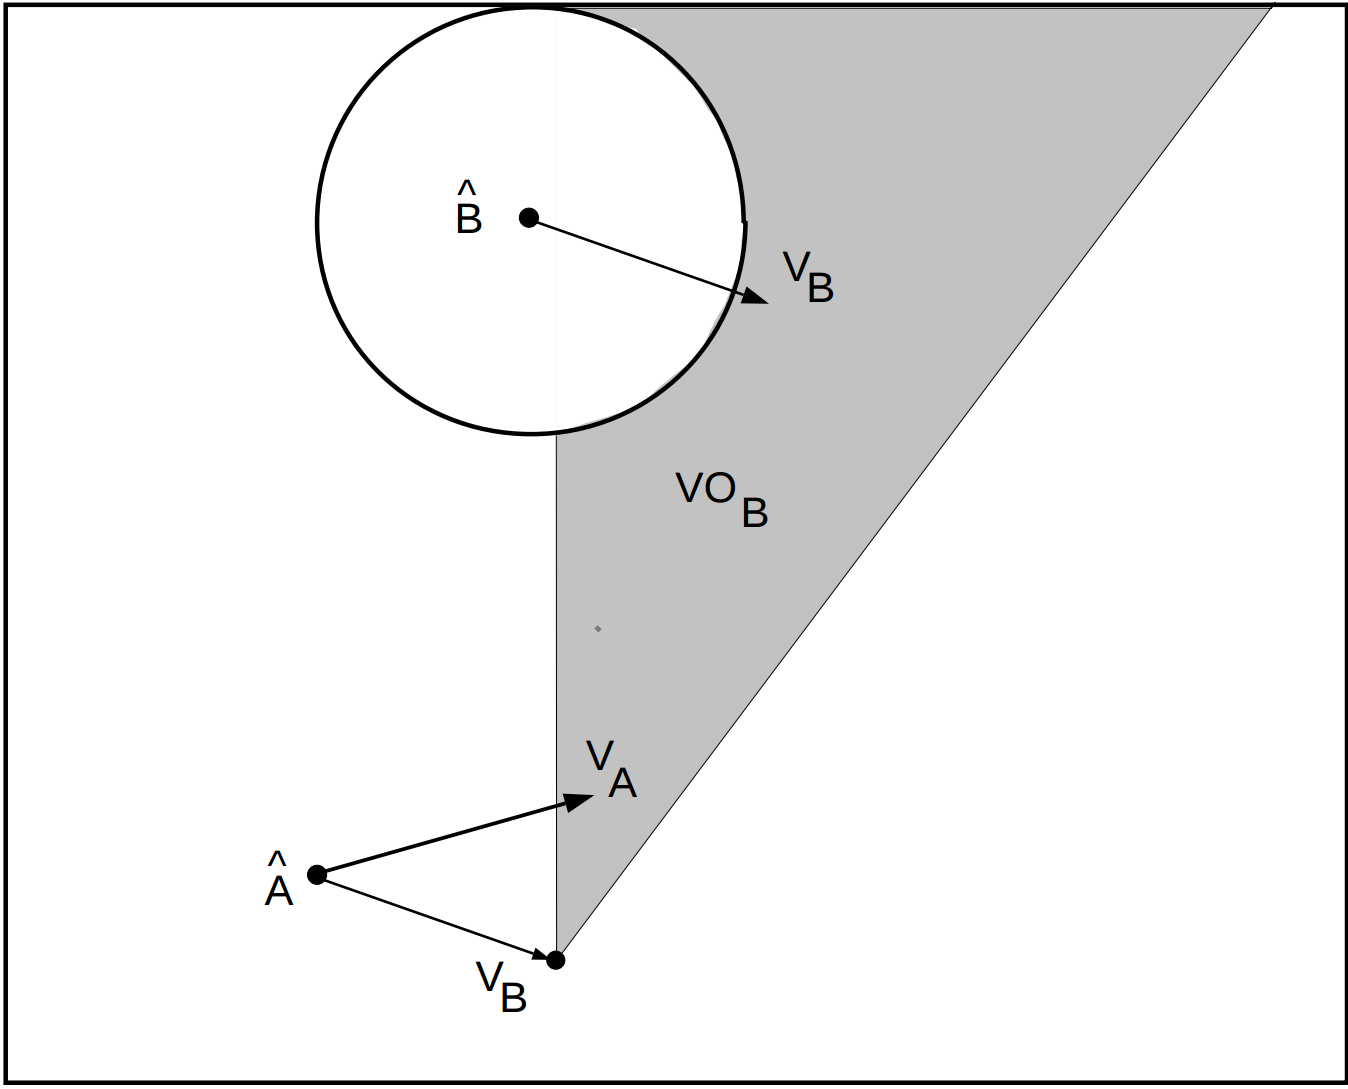
\includegraphics[width=0.6\columnwidth]{vo} 
\caption[Velocity Obstacle traslato della velocit\'a di B]{Velocity Obstacle traslato della velocit\'a di B}
\label{fig:vo} 
\end{figure}

\subsection{New velocity}
La computazione della nuova velocit\'a, in ogni time-step, deve essere selezionata fuori dal VO.
 Sfortunatamente, il concetto di Velocity Obstacle porta alla creazione di traiettorie oscillatorie sgradevoli.
 \\Pi\'u precisamente, se i robot \textit{A} e \textit{B} si stanno muovendo, rispettivamente, con {\bfseries\textit{v}\ped A} e {\bfseries\textit{v}\ped B}, si avr\'a che {\bfseries\textit{v}\ped A} $\in$ {\textit{VO}\ped {A,B}}({\bfseries\textit{v}\ped B}) e {\bfseries\textit{v}\ped B} $\in$ {\textit{VO}\ped {B,A}}( {\bfseries\textit{v}\ped A}).
 Quindi, lungo le stesse velocit\'a correnti, saranno in collisione. Perci\'o l'agente \textit{A} decider\'a di modificare la sua velocit\'a con {\bfseries\textit{v'}\ped A}, tale che sia fuori dal Velocity Obstacle di \textit{B}. Allo stesso tempo, \textit{B} modificher\'a la sua velocit\'a {\bfseries\textit{v'}\ped B}, che dovr\'a essere scelta fuori dal Velocity Obstacle di \textit{A}.
 \\Quindi, in questa nuova situazione, le vecchie velocit\'a {\bfseries\textit{v}\ped A} e {\bfseries\textit{v}\ped B} saranno fuori dal Velocity Obslacle di \textit{B} e \textit{A}, rispettivamente  {\bfseries\textit{v}\ped A} $\notin$ {\textit{VO}\ped {A,B}}({\bfseries\textit{v'}\ped B}) e  {\bfseries\textit{v}\ped B} $\notin$ {\textit{VO}\ped {B,A}}({\bfseries\textit{v'}\ped A}).
 Se entrambi gli agenti preferiscono le vecchie velocit\'a, per esempio perch\'e li porta direttamente al proprio \textit{goal}, le sceglieranno ancora. Nel ciclo successivo, queste velocit\'a si tradurranno in una collisione e loro (A e B) probabilmente sceglieranno di nuovo {\bfseries\textit{v'}\ped A} e {\bfseries\textit{v'}\ped B}, e cos\'i via.
\\Perci\'o gli agenti oscillano tra queste due velocit\'a, creando una traiettoria oscillatoria.

%%%%%%%%%%%%%%%%%%%%%%%%%%%%%%%%%%%%%%%%%%%%%%%%%%%%%%%%%%%%

% !TEX encoding = UTF-8
% !TEX TS-program = pdflatex
% !TEX root = ../Tesi.tex
% !TEX spellcheck = it-IT

%************************************************
\chapter{Reciprocal Velocity Obstacle}
\label{cap:rvo}
%************************************************

Reciprocal Velocity Obstacle affronta il problema dell'oscillazione causato dal Velocity Obstacle incorporando la natura reattiva degli altri robot.

\section{Reciprocal Velocity Obstacle}
Per affrontare il problema delle traiettorie oscillatorie, invece di dover prendere tutte le responsabilit\'a, RVO lascia prendere al robot solo la met\'a della responsabilit\'a, per evitare le collisioni, pur assumendo che l'altro robot coinvolto ricambi prendendosi cura dell'altra met\'a.
\\L'idea base sarebbe di scegliere una nuova velocit\'a per ogni agente all'esterno degli altri Velocity Obstacle e che, questa nuova velocit\'a,  sia la media (\textit{average}) della velocit\'a corrente e di una velocit\'a che sia al di fuori degli Velocity Obstacle degli altri agenti. 

\subsection{Definition}

Questo principio \'e formalizzato come segue:

\begin{gather}
RVO_{A,B}({\boldsymbol{v}_ B}, {\boldsymbol{v}_A} ) =  \{ \boldsymbol{v'}_{A} | 2\boldsymbol{v'}_{A} - \boldsymbol{v}_{A} \in VO_{A,B}(\boldsymbol{v}_{B})  \}
\end{gather}

dove RVO\ped {A,B}({\bfseries\textit{v}\ped B},{\bfseries\textit{v}\ped A}) dell'agente \textit{B} su l'agente \textit{A} contiene tutte le velocit\'a per \textit{A} che saranno la media della velocit\'a corrente {\bfseries\textit{v}\ped A} e una velocit\'a all'interno di VO\ped{A,B}({\bfseries\textit{v}\ped B}) dell'agente \textit{B}. Pu\'o essere interpretato geometricamente come Velocity Obstacle, VO\ped{A,B}({\bfseries\textit{v}\ped B}),  traslato di $\tfrac{\boldsymbol{v}_ A + \boldsymbol{v}_ B}{2}$ dall'apice.

\section{Guarantees}
Proviamo che RVO possa essere usato per generare \textit{collision-free} e \textit{oscillation-free} per ogni agente.

\subsection{Collision-free Navigation}
Abbiamo {\bfseries\textit{v}\ped A} e {\bfseries\textit{v}\ped B} velocit\'a correnti, rispettivamente, di \textit{A} e \textit{B}, e permettiamo di scegliere ad entrambi la nuova velocit\'a ({\bfseries\textit{v'}\ped A} e {\bfseries\textit{v'}\ped B}) fuori da ogni 
Reciprocal Velocity Obstacle. Rispettando il \textit{teorema} e la \textit{legge} seguenti, essi ci garantiscono uno stato di \textit{safe} se e solo se entrambi gli agenti scelgono lo stesso lato (\textit{same side}) per passare ogni altro agente. 

\begin{teorema}[Collision-Free]

$\\{\boldsymbol{v'}_ A} \overrightarrow{\notin} RVO_{A,B}({\boldsymbol{v}_ B}, {\boldsymbol{v}_A} ) \wedge {\boldsymbol{v'}_ B} \overrightarrow{\notin} RVO_{B,A}({\boldsymbol{v}_ A}, {\boldsymbol{v}_B} ) \Rightarrow {\boldsymbol{v'}_ A} \overrightarrow{\notin} VO_{A,B}({\boldsymbol{v'}_ B}) \wedge {\boldsymbol{v'}_ B} \overrightarrow{\notin} VO_{B,A}({\boldsymbol{v'}_ A}) $
\end{teorema}

\begin{figure}
\centering 
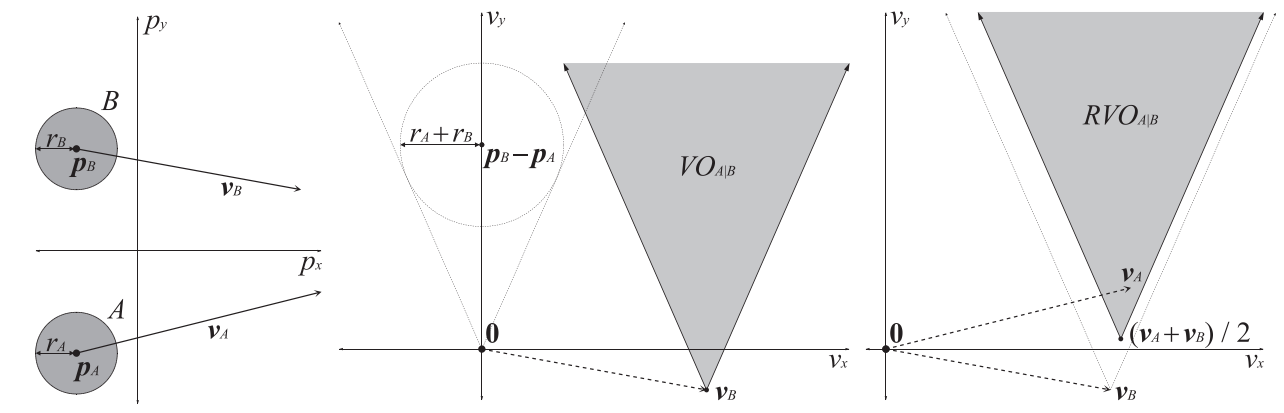
\includegraphics[width=0.8\columnwidth]{rvo} 
\caption[Costruzione del RVO rispetto al VO]{Costruzione del RVO rispetto al VO}
\label{fig:rvo} 
\end{figure}


\subsection{Same Side}
Possiamo garantire che entrambi gli agenti prenderanno automaticamente la nuova velocit\'a nello stesso lato, se ogni agente prender\'a la velocit\'a al di fuori di ogni RVO, tale che differisca del minimo possibile (\textit{closet}) dalla velocit\'a corrente dell'agente.
\\Ogni agente \textit{A} avr\'a una velocit\'a {\bfseries\textit{v}\ped A} + {\bfseries\textit{u}} \textit{closet} a {\bfseries\textit{v}\ped A} fuori dal RVO di \textit{B}, tale che B avr\'a {\bfseries\textit{v}\ped B} - {\bfseries\textit{u}} \textit{closet} a {\bfseries\textit{v}\ped B } fuori dal RVO di \textit{A}.
Se per \textit{A} questa \textit{closet} velocit\'a sar\'a sulla destra (o sinistra) di RVO di \textit{B}, allora \textit{B} sceglier\'a la \textit{closet} velocit\'a sullo stesso lato (e viceversa).\\Questo \'e provato dalla legge seguente:

\begin{legge}[Same Side]
\label{lex:sasi}
$\\ {\boldsymbol{v}_ A} + {\boldsymbol{u}} \notin RVO_{A,B}({\boldsymbol{v}_ B},{\boldsymbol{v}_ A}) \Leftrightarrow {\boldsymbol{v}_ B} - {\boldsymbol{u}} \notin RVO_{B,A}({\boldsymbol{v}_ A},{\boldsymbol{v}_ B})$
\end{legge}

\subsection{Oscillation-Free}

La scelta delle \textit{closet} velocit\'a, al di fuori degli RVO, garantisce la \textit{oscillation-free navigation} .Questo \'e provato dal teorema seguente:

\begin{teorema}[Oscillation-Free]

$\\{\boldsymbol{v}_ A} \in RVO_{A,B}({\boldsymbol{v}_ B}, {\boldsymbol{v}_A} ) \Leftrightarrow  {\boldsymbol{v}_ A} \in RVO_{A,B}({\boldsymbol{v}_ B - u }, {\boldsymbol{v}_A} + u )$
\end{teorema}

Quindi, la vecchia velocit\'a {\bfseries\textit{v}\ped A} di \textit{A} \'e all'interno del nuovo RVO di \textit{B}, dando le nuove velocit\'a {\bfseries\textit{v}\ped A} + {\bfseries\textit{u}} e {\bfseries\textit{v}\ped B} - {\bfseries\textit{u}} per l'agente \textit{A} e \textit{B}. Stesse premesse vengono rispettate per \textit{B}. 
Pertanto, dopo aver scelto la nuova velocit\'a, le vecchie candidate non saranno pi\'u valide e non verranno pi\'u scelte. Infatti, scegliendo la \textit{closet} velocit\'a fuori dal RVO di \textit{A} e di \textit{B}, gli RVO rimarranno esattamente nella stessa posizione.
Quindi {\bfseries\textit{v}\ped A} + {\bfseries\textit{u}} e {\bfseries\textit{v}\ped B} - {\bfseries\textit{u}} saranno ancora le velocit\'a pi\'u vicine alle velocit\'a preferite tra tutte quelle ammissibili. Di conseguenza non si verificheranno traiettorie oscillatorie.




% !TEX encoding = UTF-8
% !TEX TS-program = pdflatex
% !TEX root = ../Tesi.tex
% !TEX spellcheck = it-IT

%************************************************
\chapter{Hybrid Reciprocal Velocity Obstacle}
\label{cap:hrvo}
%************************************************

Con le nozioni esplicitate precedentemente per VO e RVO, HRVO permette di diminuire le oscillazioni e creare traiettorie \textit{smooth}, (osservare l'immagine del capitolo per comprendere alcuni aspetti sulla CL di RVO).

\section{Hybrid Reciprocal Velocity Obstacle}

Per l'agente {\bfseries\textit{A}} e {\bfseries\textit{B}}, se {\bfseries\textit{v}\ped {A}}  \'e sulla destra del \textit{centreline} (CL) di \textit{RVO}\ped{A,B}, il quale per simmetria {\bfseries\textit{v}\ped {B}} sar\'a sul lato destro della \textit{centreline} di \textit{RVO}\ped{B,A}, noi speriamo che \textit{A} scelga la velocit\'a sulla destra di \textit{RVO}\ped{A,B}. Per favorire questo, l' \textit{RVO} \'e allargato sostituendo il bordo sul lato dove desideriamo che il robot non passi, in questo caso il lato sinistro, dal bordo della \textit{VO}\ped{A,B}. L'apice della risultante del cono corrisponde al punto di intersezione tra il lato destro della \textit{RVO}\ped{A,B} e il lato sinistro della \textit{VO}\ped{A,B}. Se la {\bfseries\textit{v}\ped {A}} st\'a a sinistra della \textit{centreline} (CL), noi replichiamo la stessa procedura scambiando la sinistra con la destra. Per questo \'e chiamato ibrido tra RVO e VO, \textit{HRVO}\ped{A,B}.  

\subsection{New Velocity}
La computazione della nuova velocit\'a chiamata {\bfseries\textit{v}\ap{new}\ped{Ai}}, al di fuori della combinazione dei HRVO, \'e la minima distanza tra la velocit\'a corrente e la velocit\'a preferita:

\begin{gather}
v^{new}_{Ai}= argmin_ {v \notin HRVO_{Ai}} norm(v - v^{pref}_{Ai}).
\end{gather}

Per computare tale velocit\'a viene utilizzato un algoritmo chiamato ClearPath, combinando tutti gli \textit{HRVO} come intersezioni di segmenti, dove le coppie dei punti di intersezione all'interno del \textit{HRVO} vengono scartati. Le possibili velocit\'a ammissibili saranno tutte le intersezioni dei coni sul bordo di \textit{HRVO}. Aggiungendo la proiezione della velocit\'a preferita, la nuova velocit\'a sar\'a selezionata tra la minima distanza che c'\'e tra le velocit\'a ammissibili (intersezioni dei coni) e la velocit\'a preferita del robot {\bfseries\textit{v}\ap{pref}\ped{Ai}} . 
\\ Se non si riesce a trovare una possibile velocit\'a ammissibile, la procedura viene ripetuta riutilizzando l'algoritmo del ClearPath.

\begin{figure}
\centering 
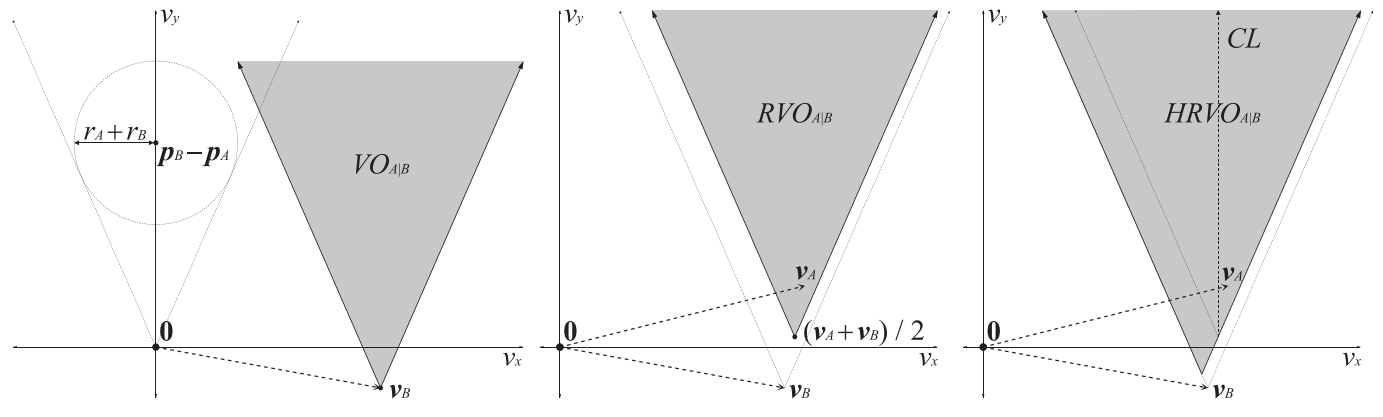
\includegraphics[width=0.8\columnwidth]{hrvo2} 
\caption[Costruzione del HRVO rispetto gli algoritmi precedentemente descritti]{Costruzione del HRVO rispetto gli algoritmi precedentemente descritti}
\label{fig:hrvo} 
\end{figure}

\subsection{Descrizione dell'algoritmo}

Descrizione dell'implementazione dell'algoritmo HRVO:
\\
\\
\begin{lstlisting}
Input A = List of robots, O = List of obstacles
loop
for all Ai in A do
Sense pAi and vAi
for all Aj E A such that j != i do
Sense pAj and vAj
Construct VOAi|Aj and RVOAi|Aj
Locate centerline CL of RVOAi|Aj
if vA is right of CL then
Replace left side of RVOAi|Aj with left side of VOAi|Aj to construct HRVOAi|Aj
else
Replace right side of RVOAi|Aj with right side of VOAi|Aj to construct HRVOAi|Aj
end if
Expand HRVOAi|Aj to HRVOAi|Aj
end for
for all Oj E O do
Sense pOj and vOj as appropriate
Construct VOAi|Oj
Expand VOAi|Oj to VOAi|Oj
end for
Construct HRVOAi from all HRVOAi|Aj and VOAi|Oj
Compute preferred velocity vprefAi
Compute new velocity vnewAi !E HRVOAi closest to vprefAi
Compute control inputs from vnewAi
Apply control inputs to actuators of Ai
end for
end loop

\end{lstlisting}












% !TEX encoding = UTF-8
% !TEX TS-program = pdflatex
% !TEX root = ../Tesi.tex
% !TEX spellcheck = it-IT

%************************************************
\chapter{Optimal reciprocal Collision Avoidance}
\label{cap:orca}
%************************************************

Optimal reciprocal Collision Avoidance \textit{ORCA} \'e un algoritmo basato su VO. 
Con questo procedimento si riduce il problema del \textit{collision-free} con una soluzione lineare computazionalmente ridotta. Ottimo anche per simulazioni popolate da centinaia di robot in uno spazio di lavoro limitato.

\section{Optimal reciprocal Collision Avoidance}

Come gli altri algoritmi precedentemente osservati, ogni robot tiene conto della velocit\'a, del raggio e della posizione corrente osservata dagli altri robot al fine di evitare collisioni. Inoltre pu\'o selezionare la sua velocit\'a dal suo spazio velocit\'a (\textit{velocity space}), dove alcune aree di questo spazio sono state etichettate come ''proibite'', per la presenza di altri robot. \\Questa formulazione, per ogni robot, crea un semipiano (\textit{half-plane}) delle velocit\'a dove è consentito essere per non avere delle collisioni. Perci\'o il robot selezioner\'a la nuova velocit\'a ottimale ({\bfseries\textit{v}\ap{opt}}) dalla intersezione di tutti i semipiani dove consentito essere. Per computare la nuova velocit\'a, si pu\'o utilizzare in modo efficente la programmazione lineare (\textit{linear programming}). In determinate condizioni, con densit\'a di robot elevate, la programmazione lineare potrebbe non trovare un risultato, in questo caso selezioniamo la pi\'u sicura velocit\'a possibile aggiungendo una terza dimensione alla programmazione lineare.

\subsection{Definition}
Dalle informazioni riportate precedentemente, selezioniamo per i robot \textit{A} e \textit{B} l'insieme delle velocit\'a permesse, che chiameremo {\bfseries\textit{V}\ped{A}} e {\bfseries\textit{V}\ped{B}}  tale che {\bfseries\textit{V}\ped{A}} sia equivalente al cono delle collisioni (${CC}_{A,B}\simeq CA^\tau_{A,B}(V_B)$) con un determinato \textit{time horizon}, {$\tau$}, che permette di creare un tronco di cono con apice nell'origine delimitato da due rette tangenti  a \textit{r}\ped a+\textit{r}\ped b, centrate in \textit{p}\ped{b} - \textit{p}\ped{a}. La dimensione della parte troncata dipende dal valore di $\tau$; il cono \'e troncato da un arco di raggio $\frac{r_a+r_b}{\tau}$ centrato in $\frac{p_b-p_a}{\tau}$. Equivalentemente per {\bfseries\textit{V}\ped{B}} tale che $CA^\tau_{B,A}(V_A)={V}_{B}$, queste aree garantiscono l'anticollisione per almeno un certo tempo $\tau$. 
\\Per ogni area viene creato un insieme di velocit\'a vicine alle velocit\'a ottimali (\textit{optimization velocities}) {\bfseries\textit{v}\ap{opt}\ped{A}} per \textit{A} e {\bfseries\textit{v}\ap{opt}\ped{B}} per \textit{B}, tale che noi denoteremo questi insiemi come \textit{ORCA}\ap{$\tau$}\ped{A,B} per \textit{A} e \textit{ORCA}\ap{$\tau$}\ped{B,A} per \textit{B}, definiti formalmente come segue:

\begin{figure}
\centering 
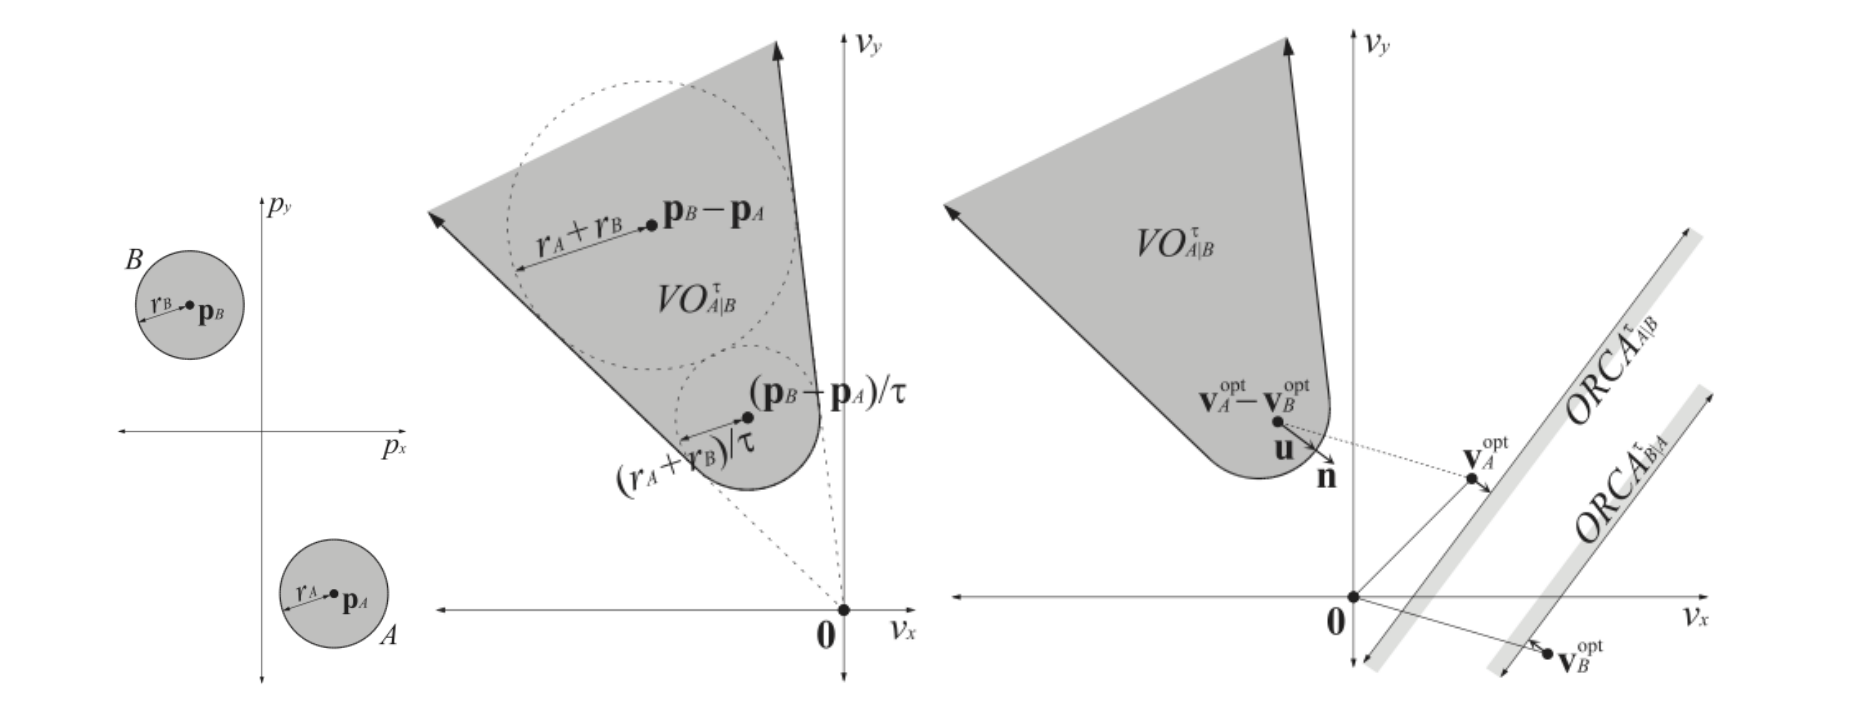
\includegraphics[width=0.8\columnwidth]{orca} 
\caption[Costruzione del cono VO\ped{A,B} con un determinato $\tau$ e la delimitazione del semipiano delle ORCA\ped{A,B} e ORCA\ped{B,A}]{Costruzione del cono VO\ped{A,B} con un determinato $\tau$ e la delimitazione del semipiano delle ORCA\ped{A,B} e ORCA\ped{B,A}}
\label{fig:orca} 
\end{figure}

\begin{definizione}[Optimal Reciprocal Collision Avoidance] 
\noindent

 \textit{ORCA}\ap{$\tau$}\ped{A,B}  e \textit{ORCA}\ap{$\tau$}\ped{B,A} sono definite reciprocamente come \textit{collision-avoiding}, tale che \textit{CA}\ap{$\tau$}\ped{A,B}(\textit{ORCA}\ap{$\tau$}\ped{B,A})$=$ \textit{ORCA}\ap{$\tau$}\ped{A,B} e \textit{CA}\ap{$\tau$}\ped{B,A}(\textit{ORCA}\ap{$\tau$}\ped{A,B})$=$ \textit{ORCA}\ap{$\tau$}\ped{B,A}, e per ogni raggio \textit{r} > 0:
\\
\\$|{ORCA}^{\tau}_{A,B} \cap D(v^{opt}_A,r)|\;=\;|{ORCA}^{\tau}_{B,A} \cap D(v^{opt}_B,r)| \\\; \;\;\;\;\;\;\;\;\;\:\geq \; \\ min(|V_A \cap D(v^{opt}_A,r)|,\:|V_B \cap D(v^{opt}_B,r)|).$
\\
\\
Questo significa che \textit{ORCA}\ap{$\tau$}\ped{A,B}  e \textit{ORCA}\ap{$\tau$}\ped{B,A} contengono pi\'u velocit\'a vicine a {\bfseries\textit{v}\ap{opt}\ped{A}} e {\bfseries\textit{v}\ap{opt}\ped{B}} che dell'insieme delle velocit\'a di \textit{collision-avoiding}.
\end{definizione} 

Possiamo costruire geometricamente \textit{ORCA}\ap{$\tau$}\ped{A,B}  e \textit{ORCA}\ap{$\tau$}\ped{B,A} assumendo che \textit{A} e \textit{B} adottino rispettivamente {\bfseries\textit{v}\ap{opt}\ped{A}} e {\bfseries\textit{v}\ap{opt}\ped{B}},  inoltre assumiamo che \textit{A} e \textit{B} siano in collisione se {\bfseries\textit{v}\ap{opt}\ped{A}} - {\bfseries\textit{v}\ap{opt}\ped{B}} $\in$ \textit{VO}\ap{$\tau$}\ped{A,B}.
Consideriamo {\bfseries\textit{u}} essere un vettore che inizia da {\bfseries\textit{v}\ap{opt}\ped{A}} - {\bfseries\textit{v}\ap{opt}\ped{B}} e punta sul punto pi\'u vicino al bordo del cono:

\begin{equation}
u=(argmin_{v \in VO^{\tau}_{A,B}}||v-(v^{opt}_{A} - v^{opt}_{B})||) - (v^{opt}_{A} - v^{opt}_{B}),
\end{equation}

assumiamo che {\bfseries\textit{n}} sia un versore che attraversa il bordo di \textit{VO}\ap{$\tau$}\ped{A,B} fino al punto ({\bfseries\textit{v}\ap{opt}\ped{A}} - {\bfseries\textit{v}\ap{opt}\ped{B}})+{\bfseries\textit{u}}. Quindi, {\bfseries\textit{u}} \'e il pi\'u piccolo cambiamento richiesto per le velocit\'a relative di \textit{A} e \textit{B}, per accorgersi della collisione al tempo $\tau$. Per spartirsi la responsabilit\'a della collisone, il robot \textit{A} adatta la sua velocit\'a per almeno $\frac{1}{2}$ {\bfseries\textit{u}} assumendo che \textit{B} si prendi cura dell'altra parte. Quindi, l'insieme delle velocit\'a permesse \textit{ORCA}\ap{$\tau$}\ped{A,B} per \textit{A}, \'e un semipiano posizionato in direzione di {\bfseries\textit{n}} con punto d'origine {\bfseries\textit{v}\ap{opt}\ped{A}}
 +$\frac{1}{2}$ {\bfseries\textit{u}}. Pi\'u nello specifico:
 
 \begin{gather}
 {ORCA}^{\tau}_{A,B} = \{ \boldsymbol{v}|( \boldsymbol{v} -(\boldsymbol{v}^{opt}_{A} + \frac{1}{2}\boldsymbol{u})) \geq 0  \}.
\end{gather}

L'insieme \textit{ORCA}\ap{$\tau$}\ped{B,A} per \textit{B} \'e definito simmetricamente. Le equazioni qui sopra riportate, si applicano anche se \textit{A} e \textit{B} non sono su una rotta di collisione quando adottano le loro velocit\'a di ottimizzazione, {\bfseries\textit{v}\ap{opt}\ped{A}}- 
{\bfseries\textit{v}\ap{opt}\ped{A}} $\notin$ \textit{VO}\ap{$\tau$}\ped{A,B}.
In questo caso, ogni robot prender\'a met\'a della responsabilit\'a per rimanere in una traiettoria di \textit{collision-free}.

\subsection{Basic Approach}

Ogni robot \textit{A} esegue un ciclo continuo di \textit{sensing} e \textit{acting} a ogni time-step $\Delta$\textit{t}. Ad ogni iterazione, i robot acquisiscono il raggio, la posizione e la velocit\'a optimale corrente degli altri robot (e di s\'e stesso). Basandosi su queste informazioni, il robot deduce il semipianio delle velocit\'a permesse,  \textit{ORCA}\ap{$\tau$}\ped{A,B}, rispettando ogni robot \textit{B}. L'insieme delle velocit\'a permesse per \textit{A}, rispetto ciascun robot, \'e l'intersezione di ogni semipiano, che noi denotiamo con \textit{ORCA}\ap{$\tau$}\ped{A}:

 \begin{gather}
 {ORCA}^{\tau}_{A} =D(0,v^{max}_{A}) \cap \bigcap_{B \neq A} ORCA^{\tau}_{A,B}
\end{gather}

Nel passo successivo, il robot seleziona la nuova velocit\'a {\bfseries\textit{v}\ap{new}\ped{A}}, per s\'e stesso, la quale sar\'a la pi\'u vicina possibile alla velocit\'a preferita {\bfseries\textit{v}\ap{pref}\ped{A}} tale che, questa velocit\'a, risiedi almeno all'interno dell'insieme delle velocit\'a permesse:

 \begin{gather}
 {v}^{new}_{A} = argmin_{v \in ORCA^{\tau}_{A}}||v-v^{pref}_{A}||.
\end{gather}

Alla prossima sezione spiegheremo come possa scegliere questa nuova velocit\'a in modo efficiente.\\ Finalmente, il robot ricever\'a la sua nuova posizione:

 \begin{gather}
 {p}^{new}_{A} = p_A + v^{new}_A\Delta t,
\end{gather}

e il ciclo di \textit{sensing-acting} verr\'a ripetuto. 
\\Per computare la nuova velocit\'a in modo efficiente, viene utilizzata la \textit{programmazione lineare}, dove \textit{ORCA}\ap{$\tau$}\ped{A} \'e una regione convessa limitata, costruita dalle intersezioni dei semipiani delle velocit\'a permesse. Se questo procedimento non porta a nessun risultato, viene aggiunta una terza dimensione, che \'e la distanza della velocit\'a preferita, cambiando il procedimento in un problema \textit{quadratico}.

\subsection{Choosing the Optimization Velocity}

Per la scelta della nuova  velocit\'a in modo efficiente:

\begin{itemize}

\item {\bfseries\textit{v}\ap{opt}\ped{A}} = 0 per ogni robot \textit{A}. Per qualsiasi robot \textit{B}, il punto 0 si trova sempre al di fuori del \textit{VO}\ap{$\tau$}\ped{A,B}. Quindi il semipiano, \textit{ORCA}\ap{$\tau$}\ped{A,B}, include sempre almeno la velocit\'a 0. Infatti la linea che delimita \textit{ORCA}\ap{$\tau$}\ped{A,B}  \'e perpendicolare alla linea che collega le posizioni attuali di \textit{A} e \textit{B}.
\\Un inconveniente, nell'impostare la nuova velocit\'a a 0, \'e che il comportamento del robot potrebbe portare ad una situazione di stallo globale, facendo convergere tutte le velocit\'a dei robot a 0, in una simulazione densamente popolata.

\item {\bfseries\textit{v}\ap{opt}\ped{A}} =  {\bfseries\textit{v}\ap{pref}\ped{A}} per ogni robot \textit{A}. La velocit\'a preferita fa parte dello stato interno di ogni robot, quindi non pu\'o essere osservata dagli altri robot. Per\'o ipoteticamente se ogni velocit\'a ottimale fosse impostata come velocit\'a preferita, per ciascun robot, questo potrebbe funzionare bene solo in un ambiente poco popolato.

\item {\bfseries\textit{v}\ap{opt}\ped{A}} =  {\bfseries\textit{v}\ped{A}} per tutti i robot \textit{A}. Impostare la velocit\'a corrente come velocit\'a ottimale, sarebbe il comportamento ideale tra le scelte elencate precedentemente. 
La  velocit\'a corrente si adatta automaticamente alla situazione, essa sar\'a pi\'u vicina alla velocit\'a preferita in ambienti di bassa densit\'a mentre sar\'a pi\'u vicina allo 0 in caso di ambienti ad alta densit\'a. Soprattutto la velocit\'a corrente pu\'o essere osservata dagli altri robot. 
\\Purtroppo la programmazione lineare potrebbe fallire in condizioni di alta densit\'a. Perci\'o la velocit\'a \textit{collision-free} non pu\'o essere garantita.
Inoltre come precedentemente anticipato, viene utilizzata una dimensione in pi\'u portando il problema in 3-D \textit{linear program}.
\end{itemize}

% !TEX encoding = UTF-8
% !TEX TS-program = pdflatex
% !TEX root = ../Tesi.tex
% !TEX spellcheck = it-IT

%************************************************
\chapter{Detect Velocity Obstacle}
\label{cap:dvo}
%************************************************

In questo capitolo introduco l'algoritmo da me implementato in Matlab, basandomi sulla libreria RVO2 v2.0.2 scritta in C++, studiata e implementatata da \textit{Jur van den Berg, Stephen J. Guy, Jamie Snape, Ming C. Lin, and Dinesh Manocha del Department of Computer Science, University of North Carolina at Chapel Hill}.
\\Nel primo affronto del problema, lo scopo era di interpretare e riscrivere la libreria, sopra citata, in Matlab;  purtroppo per alcuni problemi implementativi (\textit{linear program e quadratic program}) ho dovuto tenere conto di alcuni aspetti fondamentali e aggirare il problema realizzando un ibrido tra RVO e HRVO, prima esplicitato, che ho chiamato \textit{Detect Velocity Obstacle}.

\section{Detect Velocity Obstacle}
DVO rispecchia l'andamento ciclico di \textit{sensing-acting} per ogni robot, questi  hanno quindi la possibilit\'a di osservare la velocit\'a, il raggio e la posizione corrente di ogni robot a ogni time-step della simulazione. 

\subsection{Struttura di ogni agente}
Le propriet\'a di ogni agente, prevedono:

\begin{itemize}
%Dove:
\item \textit{Identity} \'e un numero che identifica l'agente.
%\begin{comment}
\item \textit{Position} rappresenta la posizione corrente dell'agente, informazione condivisa agli altri agenti.
\item \textit{Target} rappresenta la posizione finale \textit{goal}, informazione \underline{non} condivisa agli altri agenti.
\item \textit{Speed} rappresenta la velocit\'a corrente, informazione condivisa agli altri agenti.
\item \textit{PrefSpeed} rappresenta la velocit\'a preferita, informazione \underline{non} condivisa agli altri agenti.
\item \textit{Radius} rappresenta il raggio dell'agente, informazione condivisa a ogni agente.
\item \textit{New\_Position} rappresenta la nuova posizione dell'agente, informazione viene condivisa a ogni agente nel ciclo successivo.
\item \textit{New\_Speed} rappresenta la nuova velocit\'a computata, sar\'a condivisa con gli altri agenti nel ciclo successivo.
\item \textit{NeighborDist} rappresenta le distanze tra i robot, informazione \underline{non}  condivisa agli altri agenti, calcolata conoscendo la posizione corrente di s\'e stesso e degli altri agenti nella scena.
%\end{comment}
\end{itemize}

\begin{lstlisting}
%%% creazione di un oggetto/classe Agente
classdef Agent < handle

% properties: instanza di ogni agente
    properties
        Identity
        Position
        Target
        Speed
        PrefSpeed
        Radius
        New_Position
        New_Speed
        NeighborDist
    end

% methods: metodi della classe Agente
    methods ( Access = public )
    
% costruttore
        function obj = Agent( id, pos, goal, vel, p_vel, rad, n_p, n_s, n_d, F )
            if nargin > 0
                for i=1:F
                    
                    obj(i).Identity = id;
                    obj(i).Position = pos;
                    obj(i).Target = goal;
                    obj(i).Speed = vel;
                    obj(i).PrefSpeed = p_vel;
                    obj(i).Radius = rad;
                    obj(i).New_Position = n_p;
                    obj(i).New_Speed = n_s;
                    obj(i).NeighborDist = n_d;
                
                end
            end
        end
        ...
\end{lstlisting}


\subsection{Find Velocity}
Per la computazione della nuova velocit\'a, la funzione di \textit{Agent.m}, \textit{$findVelocity(obj,others,time)$} prende in input l'agente \textit{A}=\textit{obj}, gli altri agenti \textit{B}\ped{i}=\textit{others} e \textit{time-step}=\textit{time}. Rappresenta la funzione principale perch\'e in essa vengono utilizzate le funzioni per il calcolo dei coni, delle velocit\'a ammissibili, l'aggiornamento della nuova velocit\'a e della nuova posizione e di conseguenza anche della velocit\'a preferita.
\textit{Admin\_Speeds(obj,time)} \'e una funzione che restituisce tutte le possibili velocit\'a ammissibili, \textit{ad\_vel}, che l'agente pu\'o selezionare in quel determinato istante temporale; in seguito viene fornita una spiegazione pi\'u formale.
 
\begin{lstlisting}
% funzione che calcola la nuova velocit\'a
    function findVelocity(obj,others,time)
            speed_ok=0;
            ad_vel=[];
            % calcolo le ammissibili velocit\'a
            ad_vel=Admin_Speeds(obj,time);
            ...
 \end{lstlisting}
 
 In seguito vengono costruiti tutti i coni che delimitano tutte le velolcit\'a che portano a una collisione con un ostacolo. Con la funzione
 \textit{cone\_VO(obj,others(i),time)} si calcolano i coni traslati delle velocit\'a dell'altro agente preso in osservazione, diviso 2 \textit{(other.Speed*time)/2}. Successivamente vengono riportati i cicli per selezionare tutte le velocit\'a esterne ai coni precedentemente calcolati.
Alla fine la funzione restituir\'a un array con tutte le velocit\'a considerate \textit{safe}.

 \begin{lstlisting}
	    ...
            for i=1:length(others)
            	% se non sono lo stesso agente
                if(others(i).Identity ~= obj.Identity)
                        % calcolo il cono delle collisioni
                        [cone]=cone_VO(obj,others(i),time); 
                        % controllo se le velocit\'a ammissibili sono dentro
                        % o fuori al cono delle collisioni
                        in=inpolygon(ad_vel(:,1),ad_vel(:,2),cone(1,:),cone(2,:));
                        ad_vel=[ad_vel,in];
                        for q=1:length(ad_vel(:,end))
                            if ad_vel(q,4) == 1
                                ad_vel(q,:)=[0,0,0,0];
                            end
                        end
                        ad_vel( all(~ad_vel,2), : ) = [];                     
                        % ritorno le velocit\'a ammissibili con la relativa
                        % distanza tra la sua v_pref
                        ad_vel=ad_vel(:,1:3);
                       speed_ok=1;
                end    
            end
            ...
\end{lstlisting}
 
 Una volta instanziato l'array \textit{ad\_vel}, estraggo la velocit\'a che differisce il meno possibile dalla distanza della velocit\'a preferita dell'agente \textit{obj}. Successivamente viene aggiornata la posizione e  la nuova velocit\'a appena calcolata. Infine aggiorno la nuova velocit\'a preferita con  gli aggiornamenti appena riportati. 
\\
\begin{lstlisting}
	    ...
            if speed_ok == 1
            
            	% estraggo da ad_vel la pi\'u piccola distanza tra v_pref e velocit\'a ammissibile    
            	[values,index]=min(ad_vel(:,3));
            
            	% setto la nuova posizione e velocit\'a
            	obj.New_Position=ad_vel(index,1:2);    
            	obj.New_Speed=(obj.New_Position-obj.Position)/time;
           
            	% aggiorno la nuova posizione
            	obj.New_Position(1) = (obj.Position(1) + obj.New_Speed(1)*time);
            	obj.New_Position(2) = (obj.Position(2) + obj.New_Speed(2)*time);
            end
            
            % aggiorno la velocit\'a preferita
            setNewPrefSpeed(obj);   
    end
end 
\end{lstlisting}

\subsection{Admissible velocity}
In questa sezione, riporto parte del codice della creazione dei possibili candidati a velocit\'a ammissibili.
\\La funzione \textit{up\_down} permette di tenere tutte le veloci\'a a destra o a sinistra della velocit\'a preferita dell'agente.

\begin{lstlisting}
...
% determino se un punto si trova a destra o a sinistra della velocit\'a preferit\'a di obj (tengo solo velocit\'a a destra della v_pref)
for i=1:numel(right_velocity)/2
    Possible_velocity=right_velocity(i,:);
    is_up=up_down(Possible_velocity,obj.Position,v_pref);
    flag(i)=is_up;
end
...
 \end{lstlisting}
 
 \newpage
 \subsection{Risultati}
Riporto le stampe delle traiettorie di alcune simulazioni.\\
Nella figura 5.1(a) mi sono posto il problema di un collision-avoidance tra due agenti che si scambiano la posizone di A con il target di B (bug riportato della librery RVO2\_ORCA).
\begin{itemize}
\item Nella figura 5.1(b) viene riportata l'immagine delle traiettorie descritte da sei agenti con lo stesso raggio, uguale a 1.3, in una configurazione a circonferenza di raggio 10 .
\item Nella figura 5.1(c) si riporta la stessa configurazione a circonferenza per\'o con il doppio degli agenti e con l'aggiunta della possibilit\'a di settare i raggi a piacimento.
\item Nella figura 5.1(d) viene configurata una simulazione dove i due agenti pi\'u esterni si devono scambiare la posizione del target rispetto l'agente verde. 
\end{itemize}
\begin{figure}
\centering
\subfloat[Due agenti di raggio 2]
{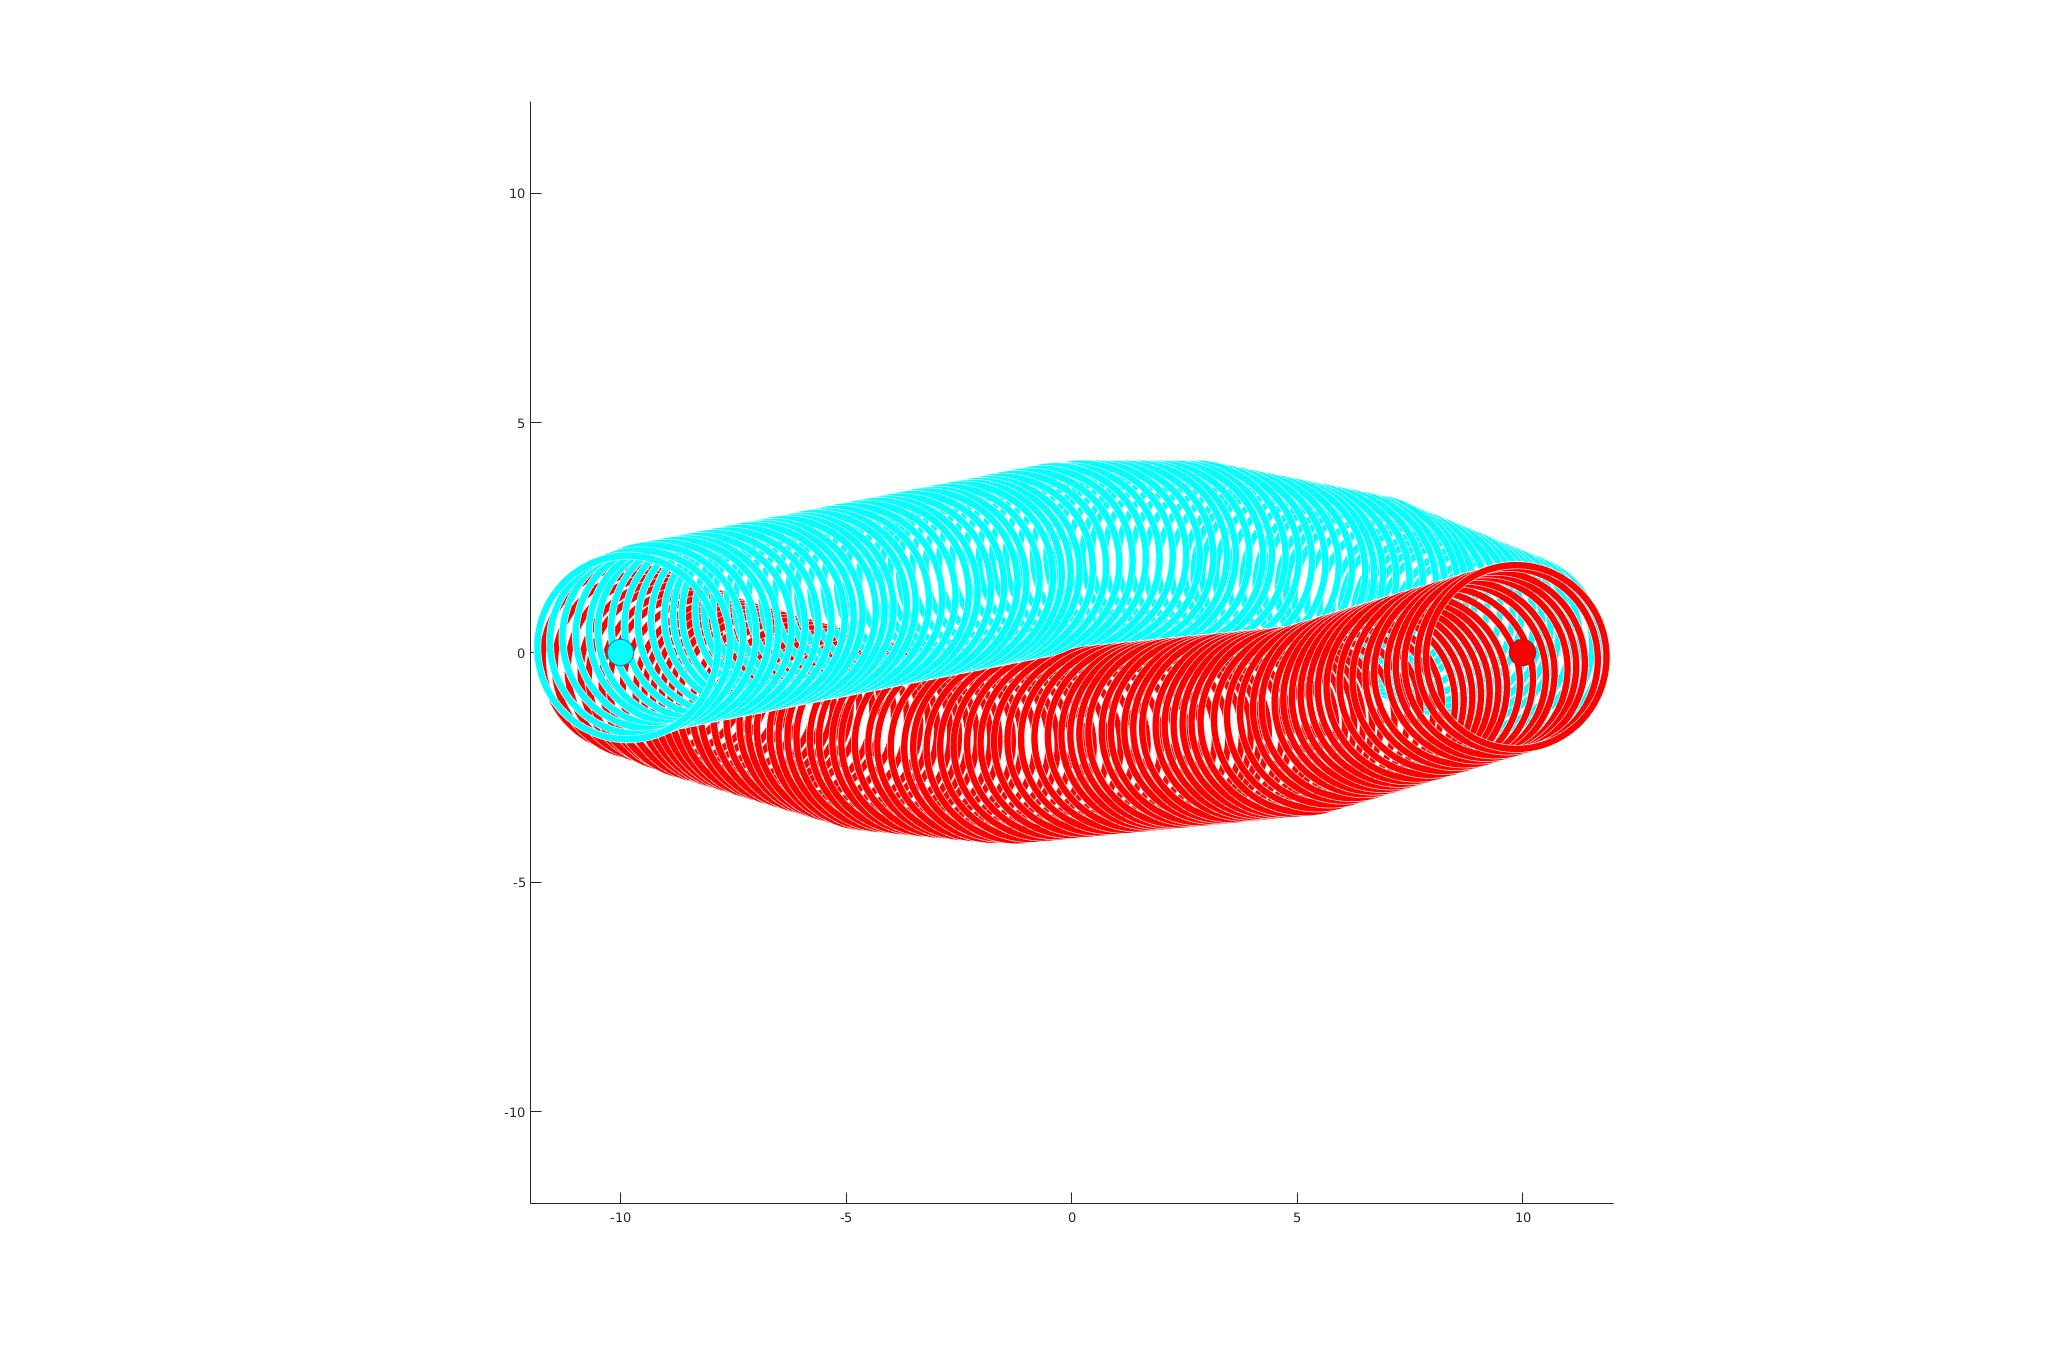
\includegraphics[width=.48\columnwidth]{Due}} \quad
\subfloat[Sei agenti di raggio 1]
{\label{fig:}
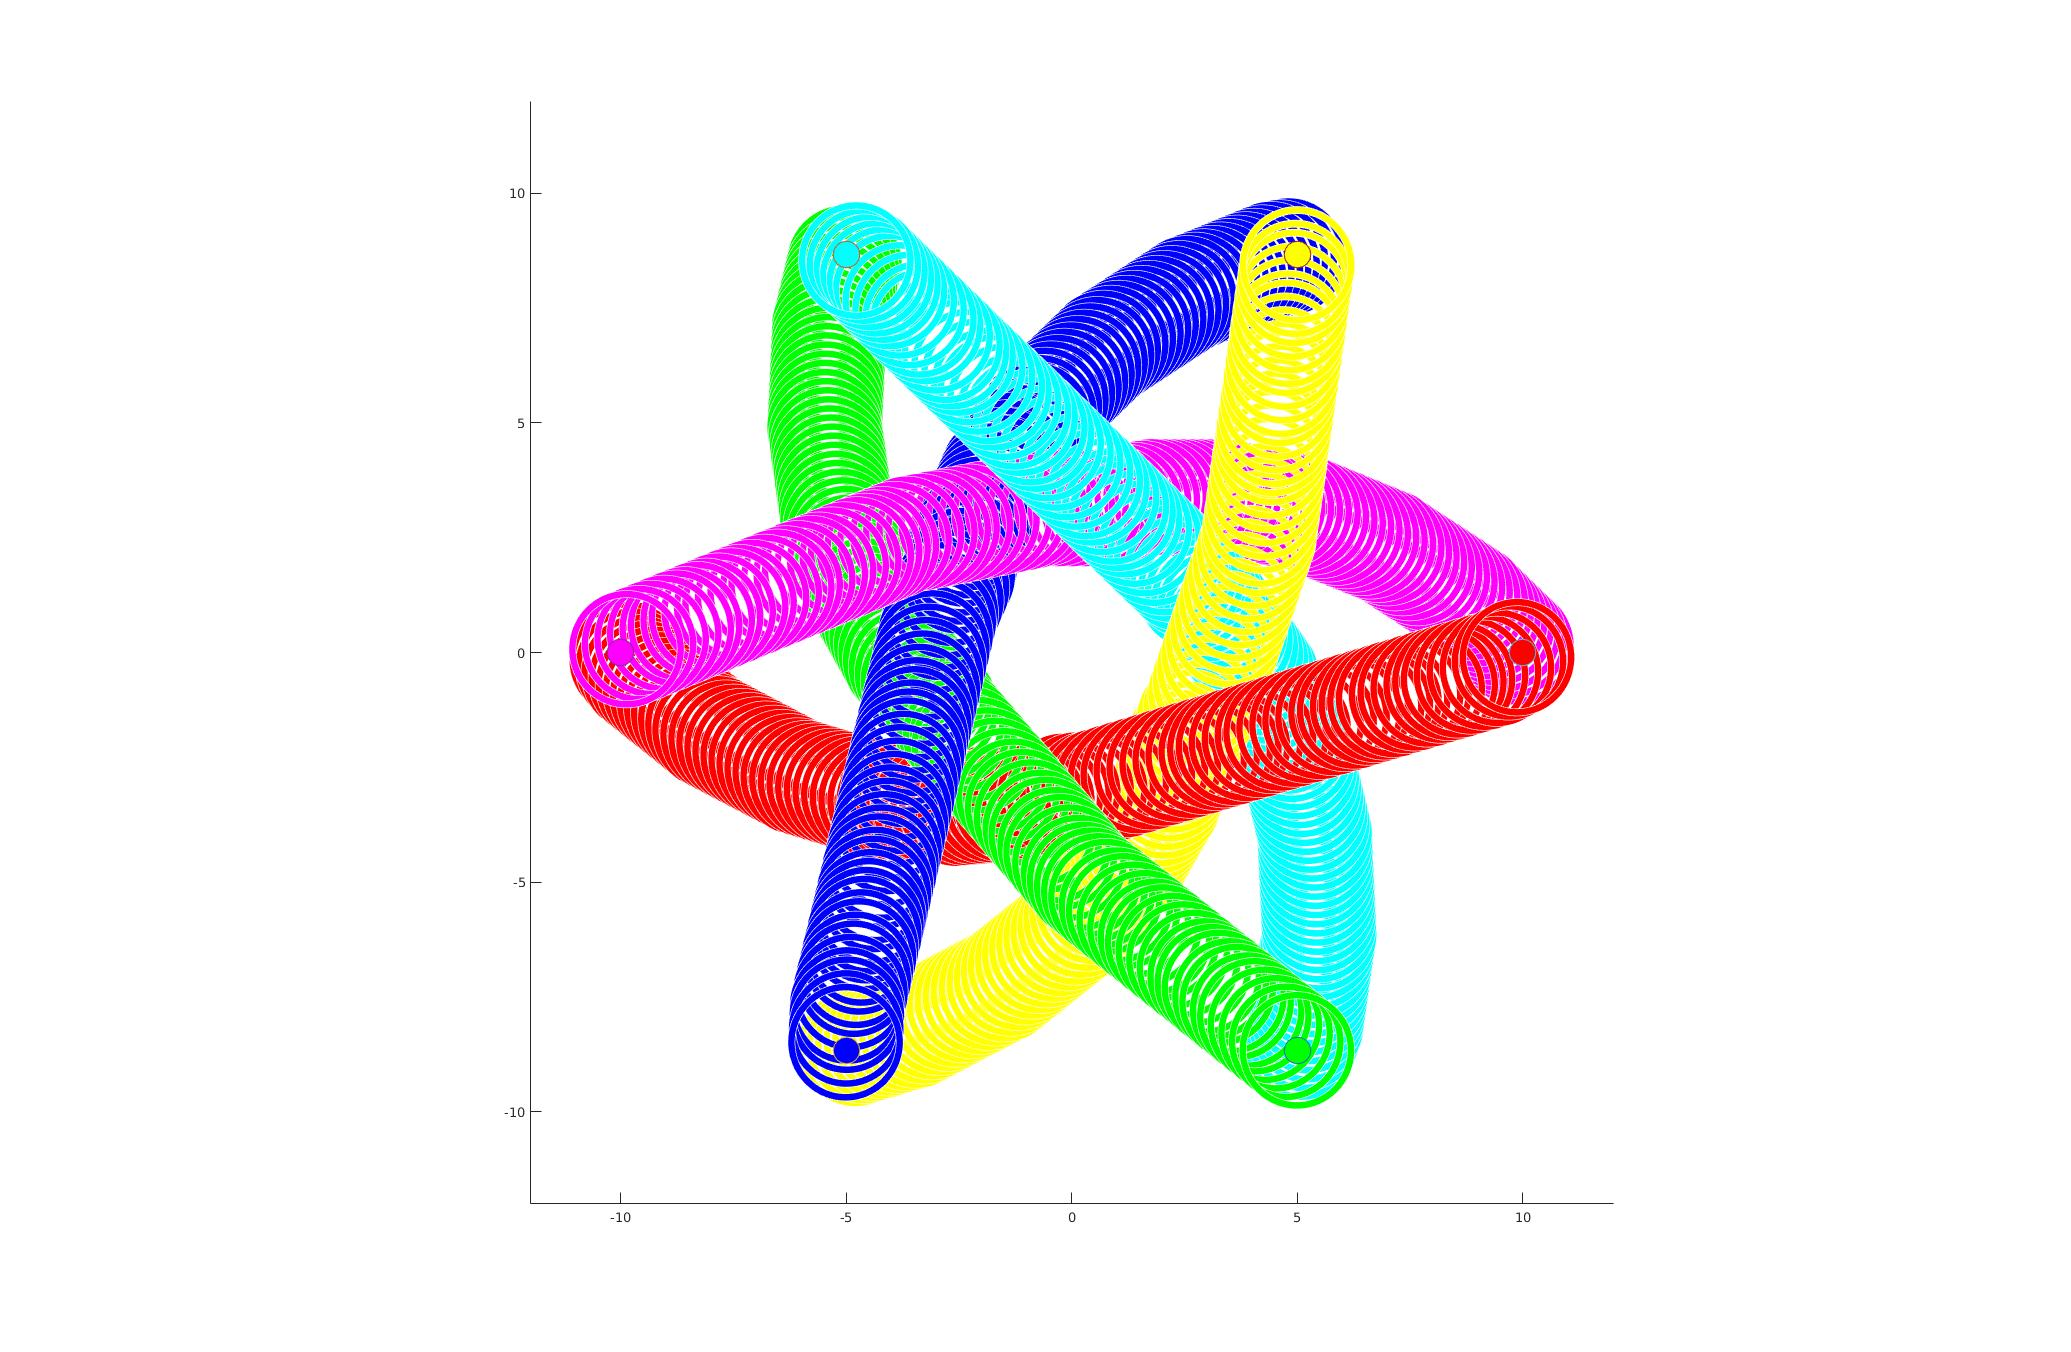
\includegraphics[width=.48\columnwidth]{sei}} \\
\subfloat[Dodici agenti di raggio random]
{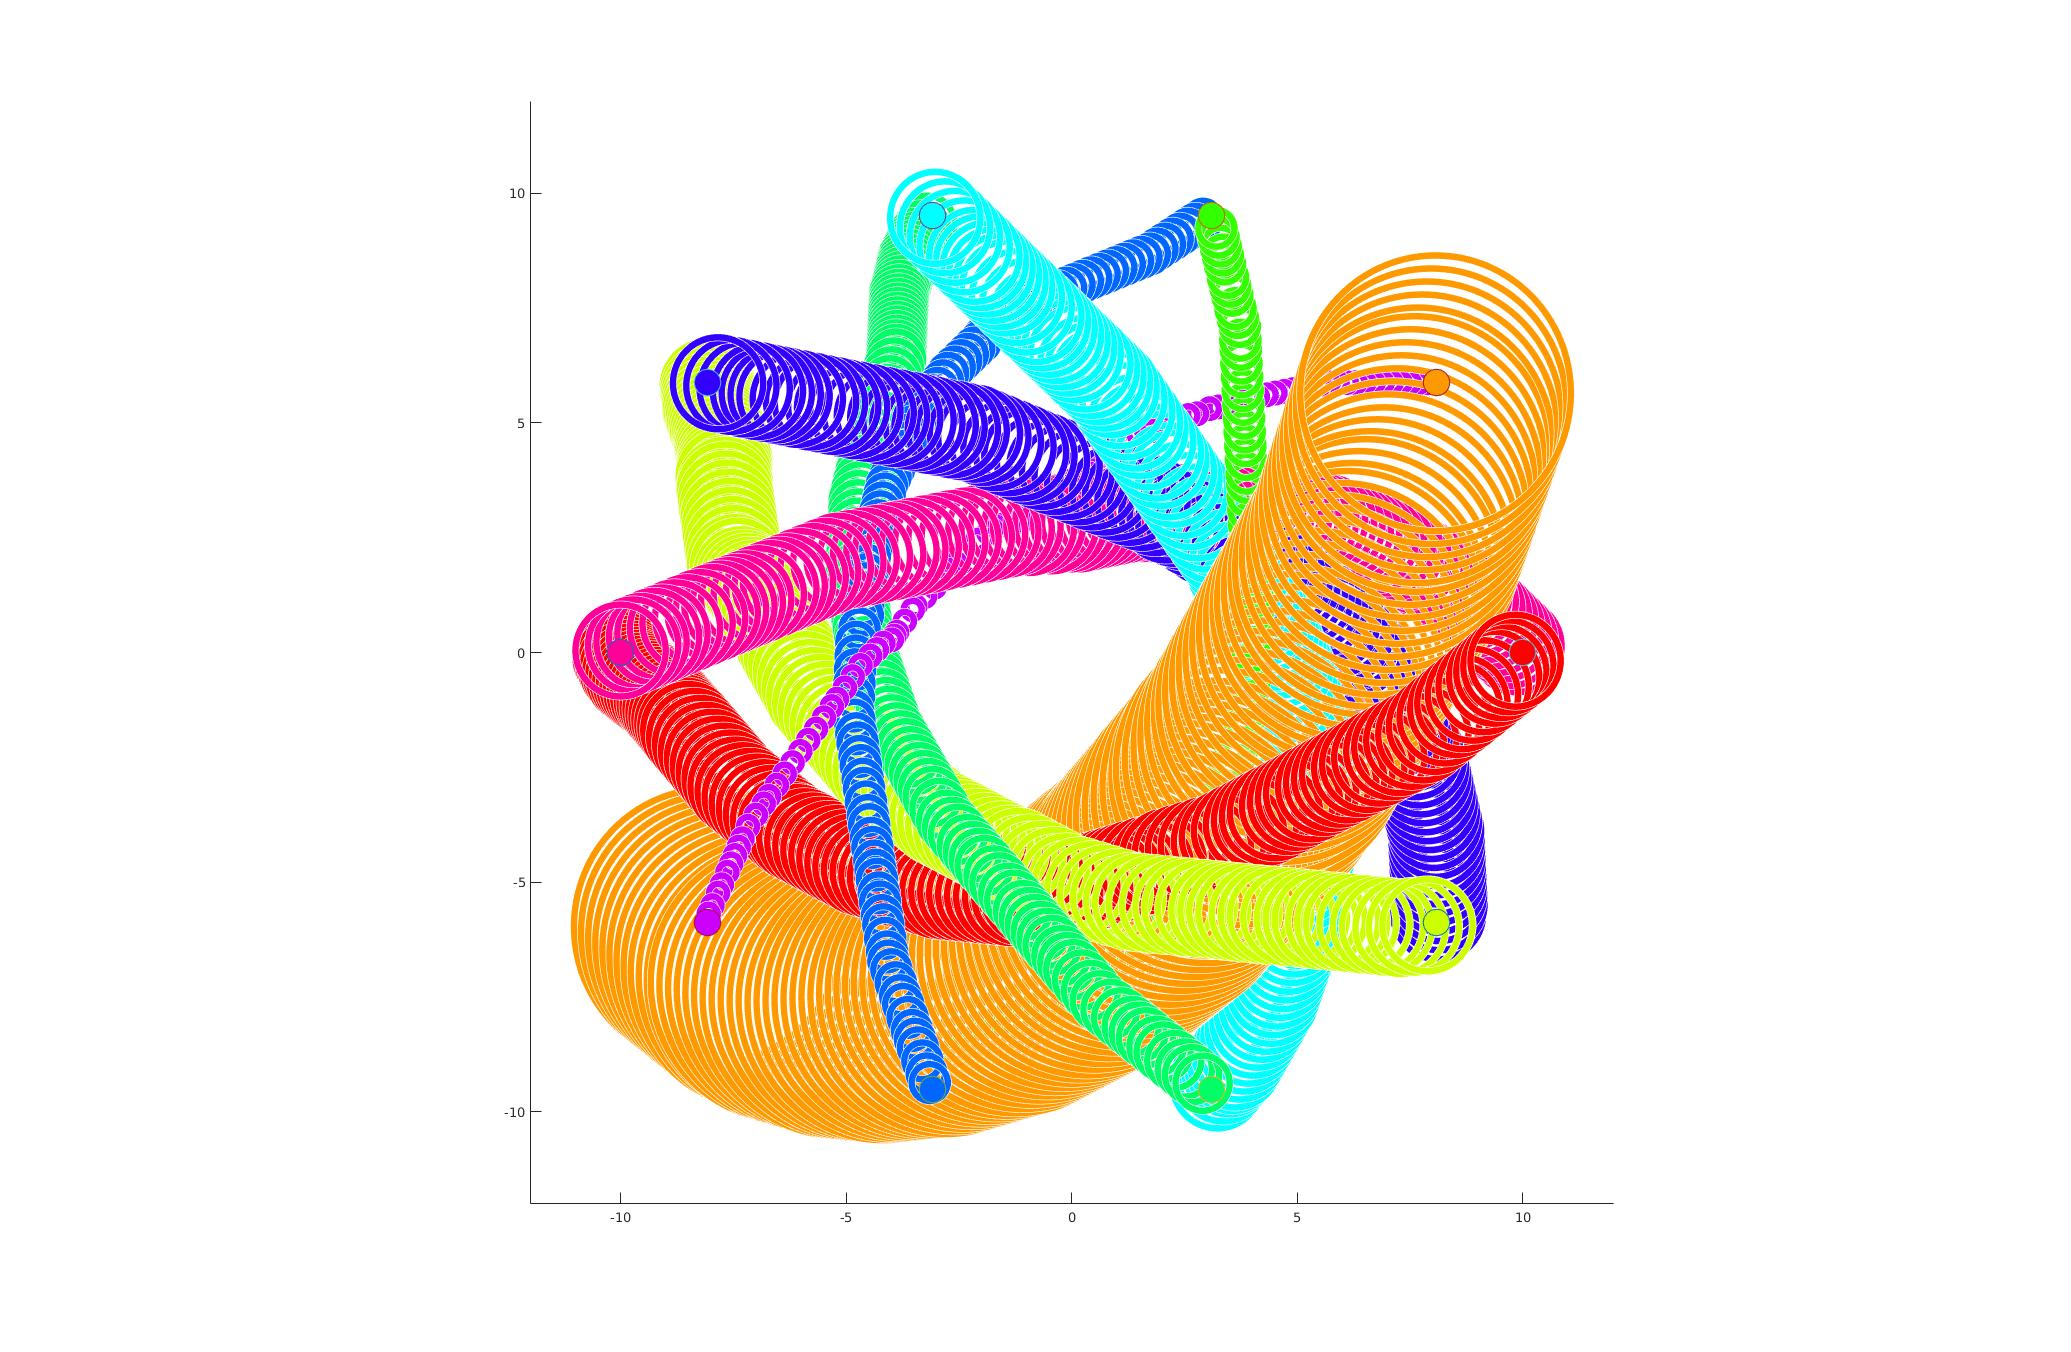
\includegraphics[width=.48\columnwidth]{random}} \quad
\subfloat[Tre agenti di raggio 1]
{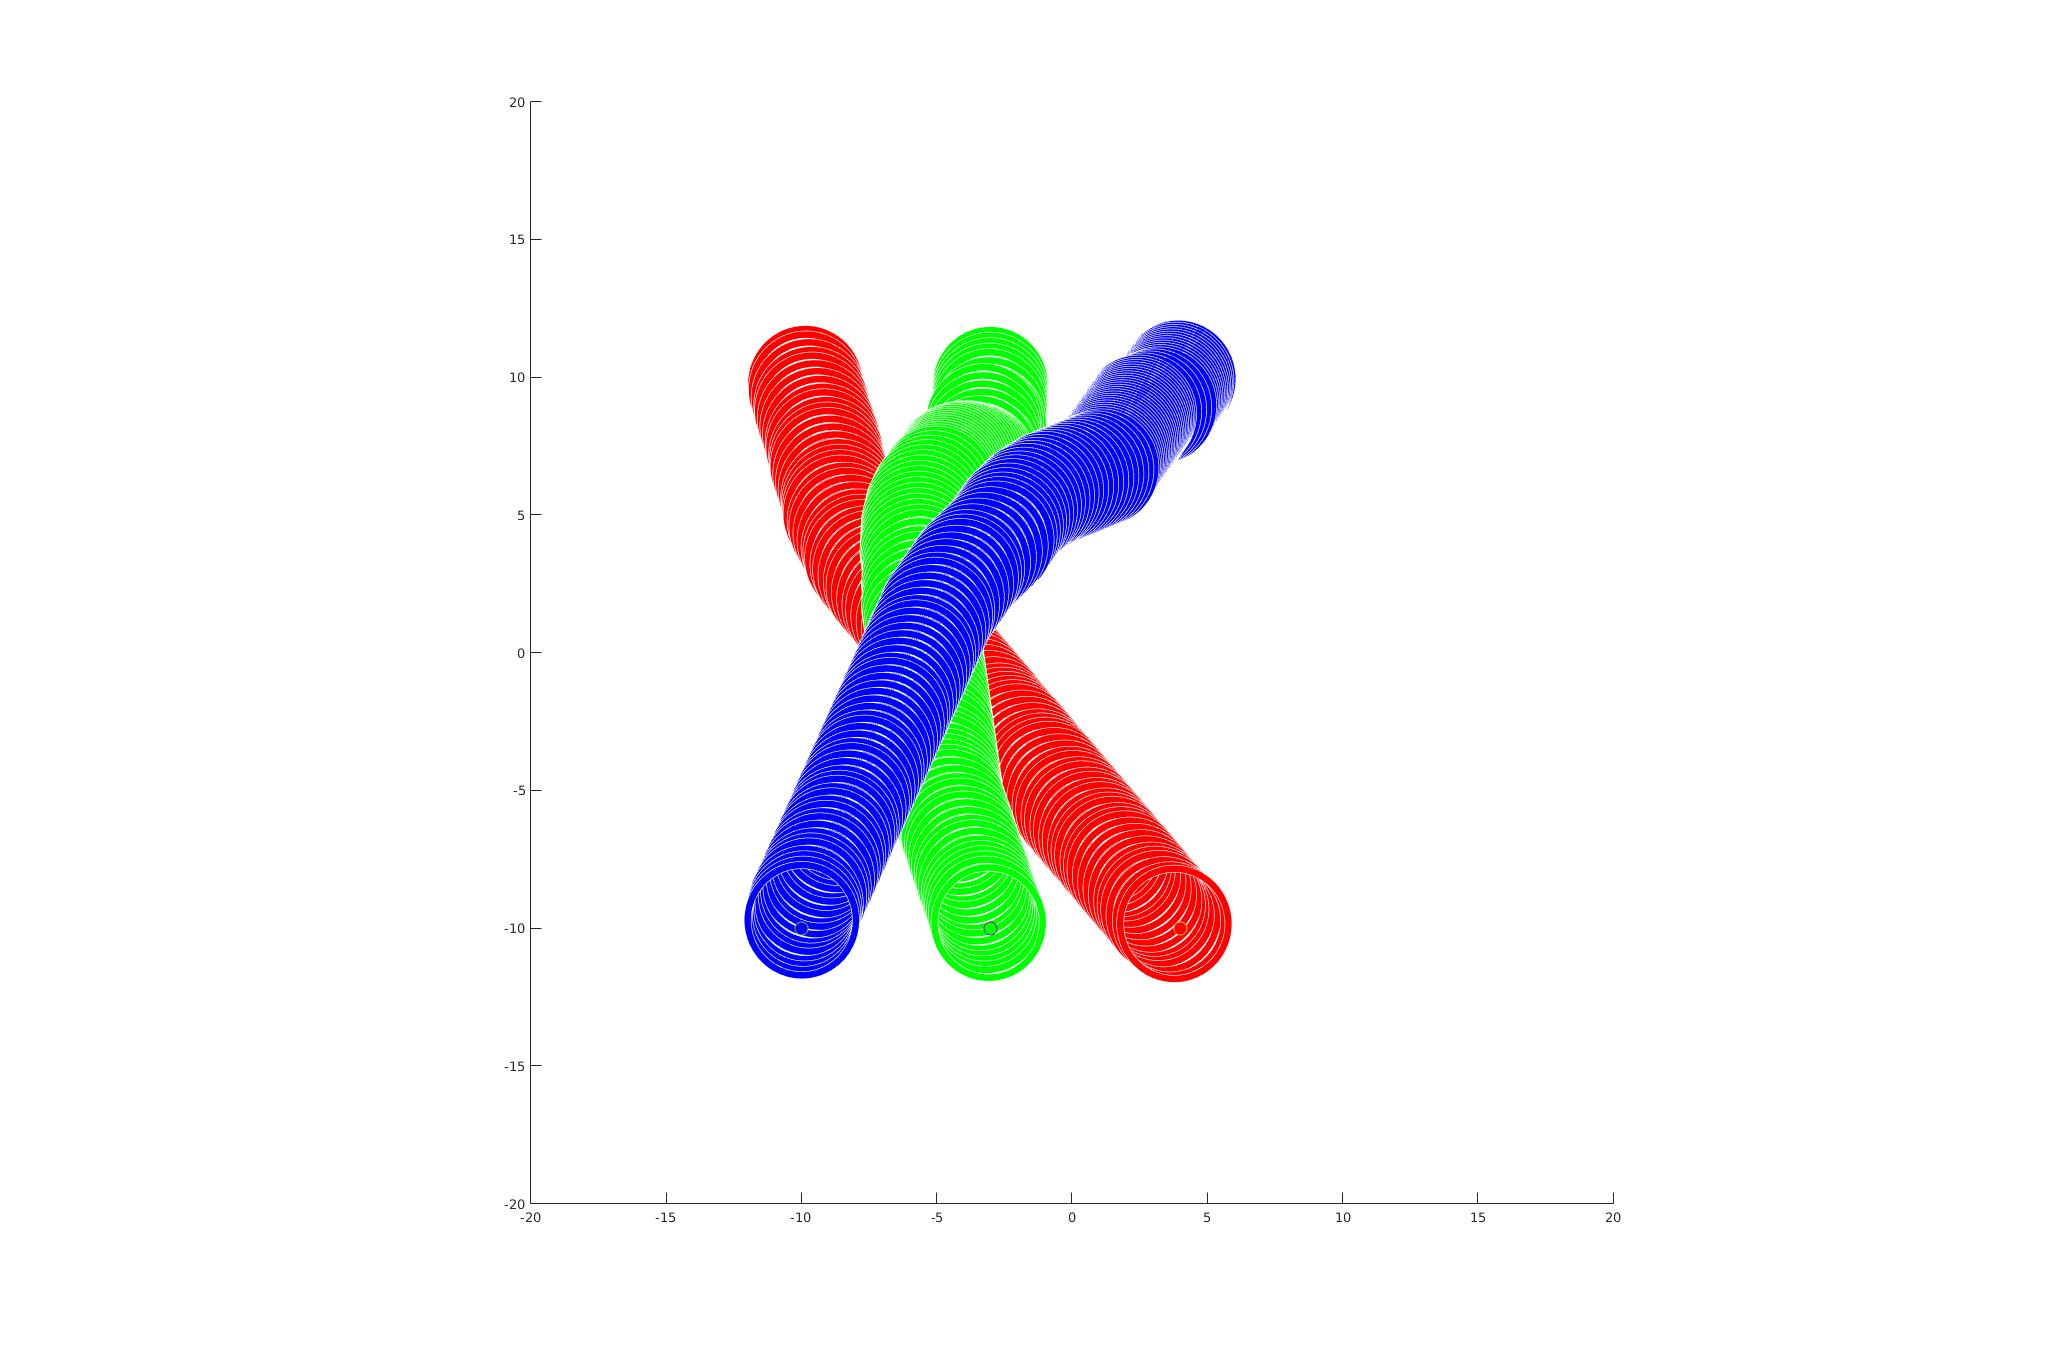
\includegraphics[width=.48\columnwidth]{X3}}
\caption[a,b,c,d dei risulati della simulazione]{Stampa delle traiettorie della simulazione}
\label{fig:}
\end{figure}
\newpage
\subsection{Risulati con $\tau$}
Mi sono posto lo stesso problema con l'aggiunta di utilizzare un cono troncato utilizzato nelle ORCA, questi sono i risultati:
\begin{itemize}
\item le traiettorie sono pi\'u rettilinee.
\item gli agenti nella parte centrale sono pi\'u vicini rispetto a non utilizzarlo.
\item con l'aumento di densit\'a della popolazione della scena \'e meglio utilizzare un $\tau$ maggiore di 2.
\end{itemize}



\begin{figure}
\centering
\subfloat[Due agenti di raggio 2]
{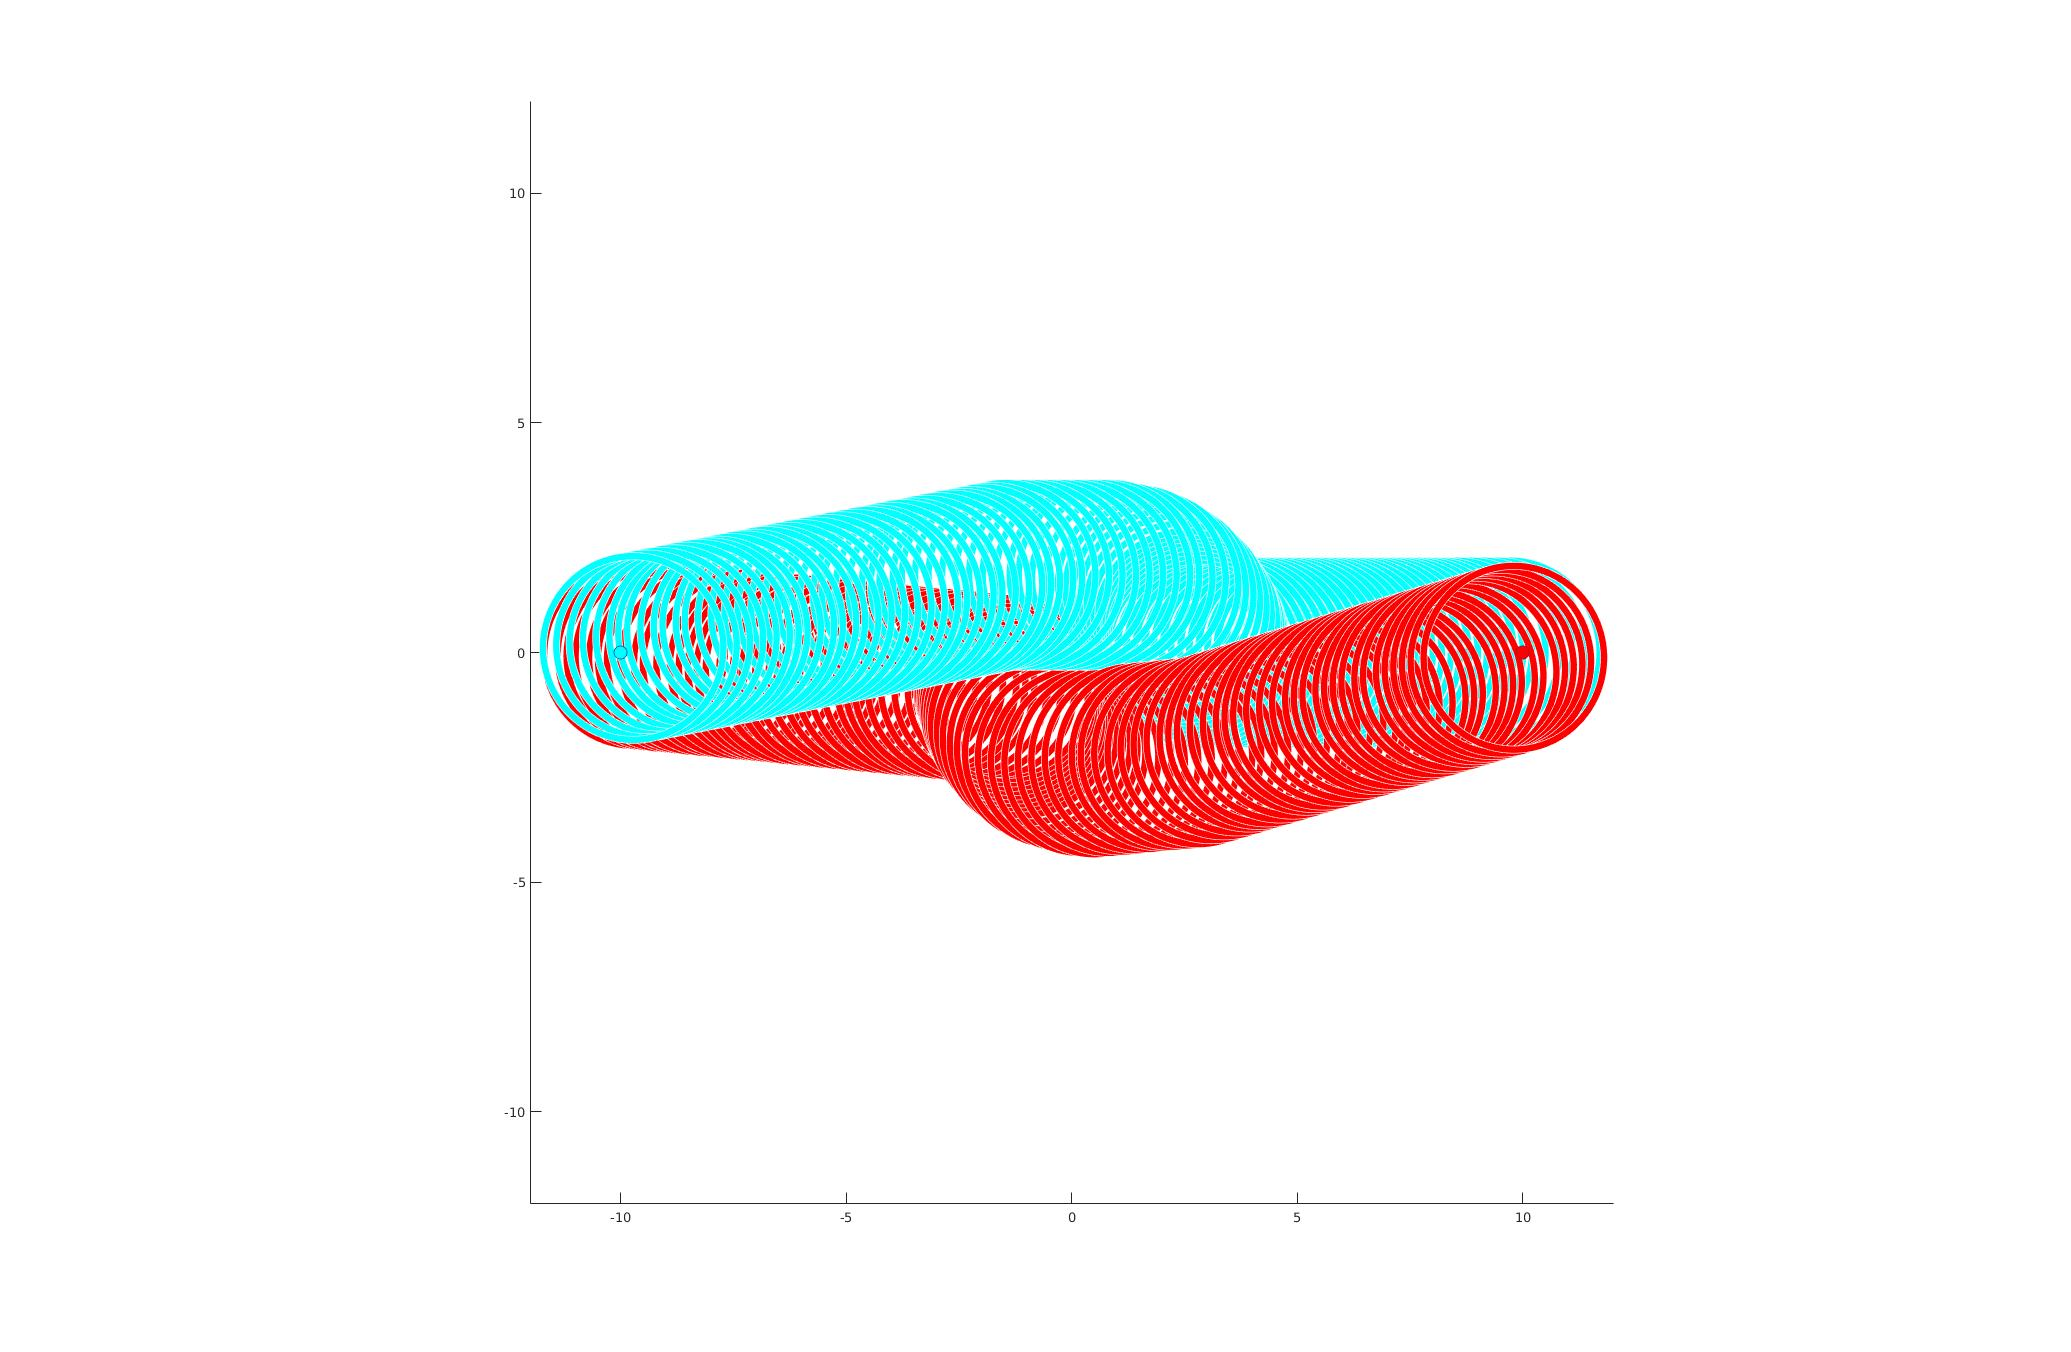
\includegraphics[width=.48\columnwidth]{2tau}} \quad
\subfloat[Sei agenti di raggio 1]
{\label{fig:}
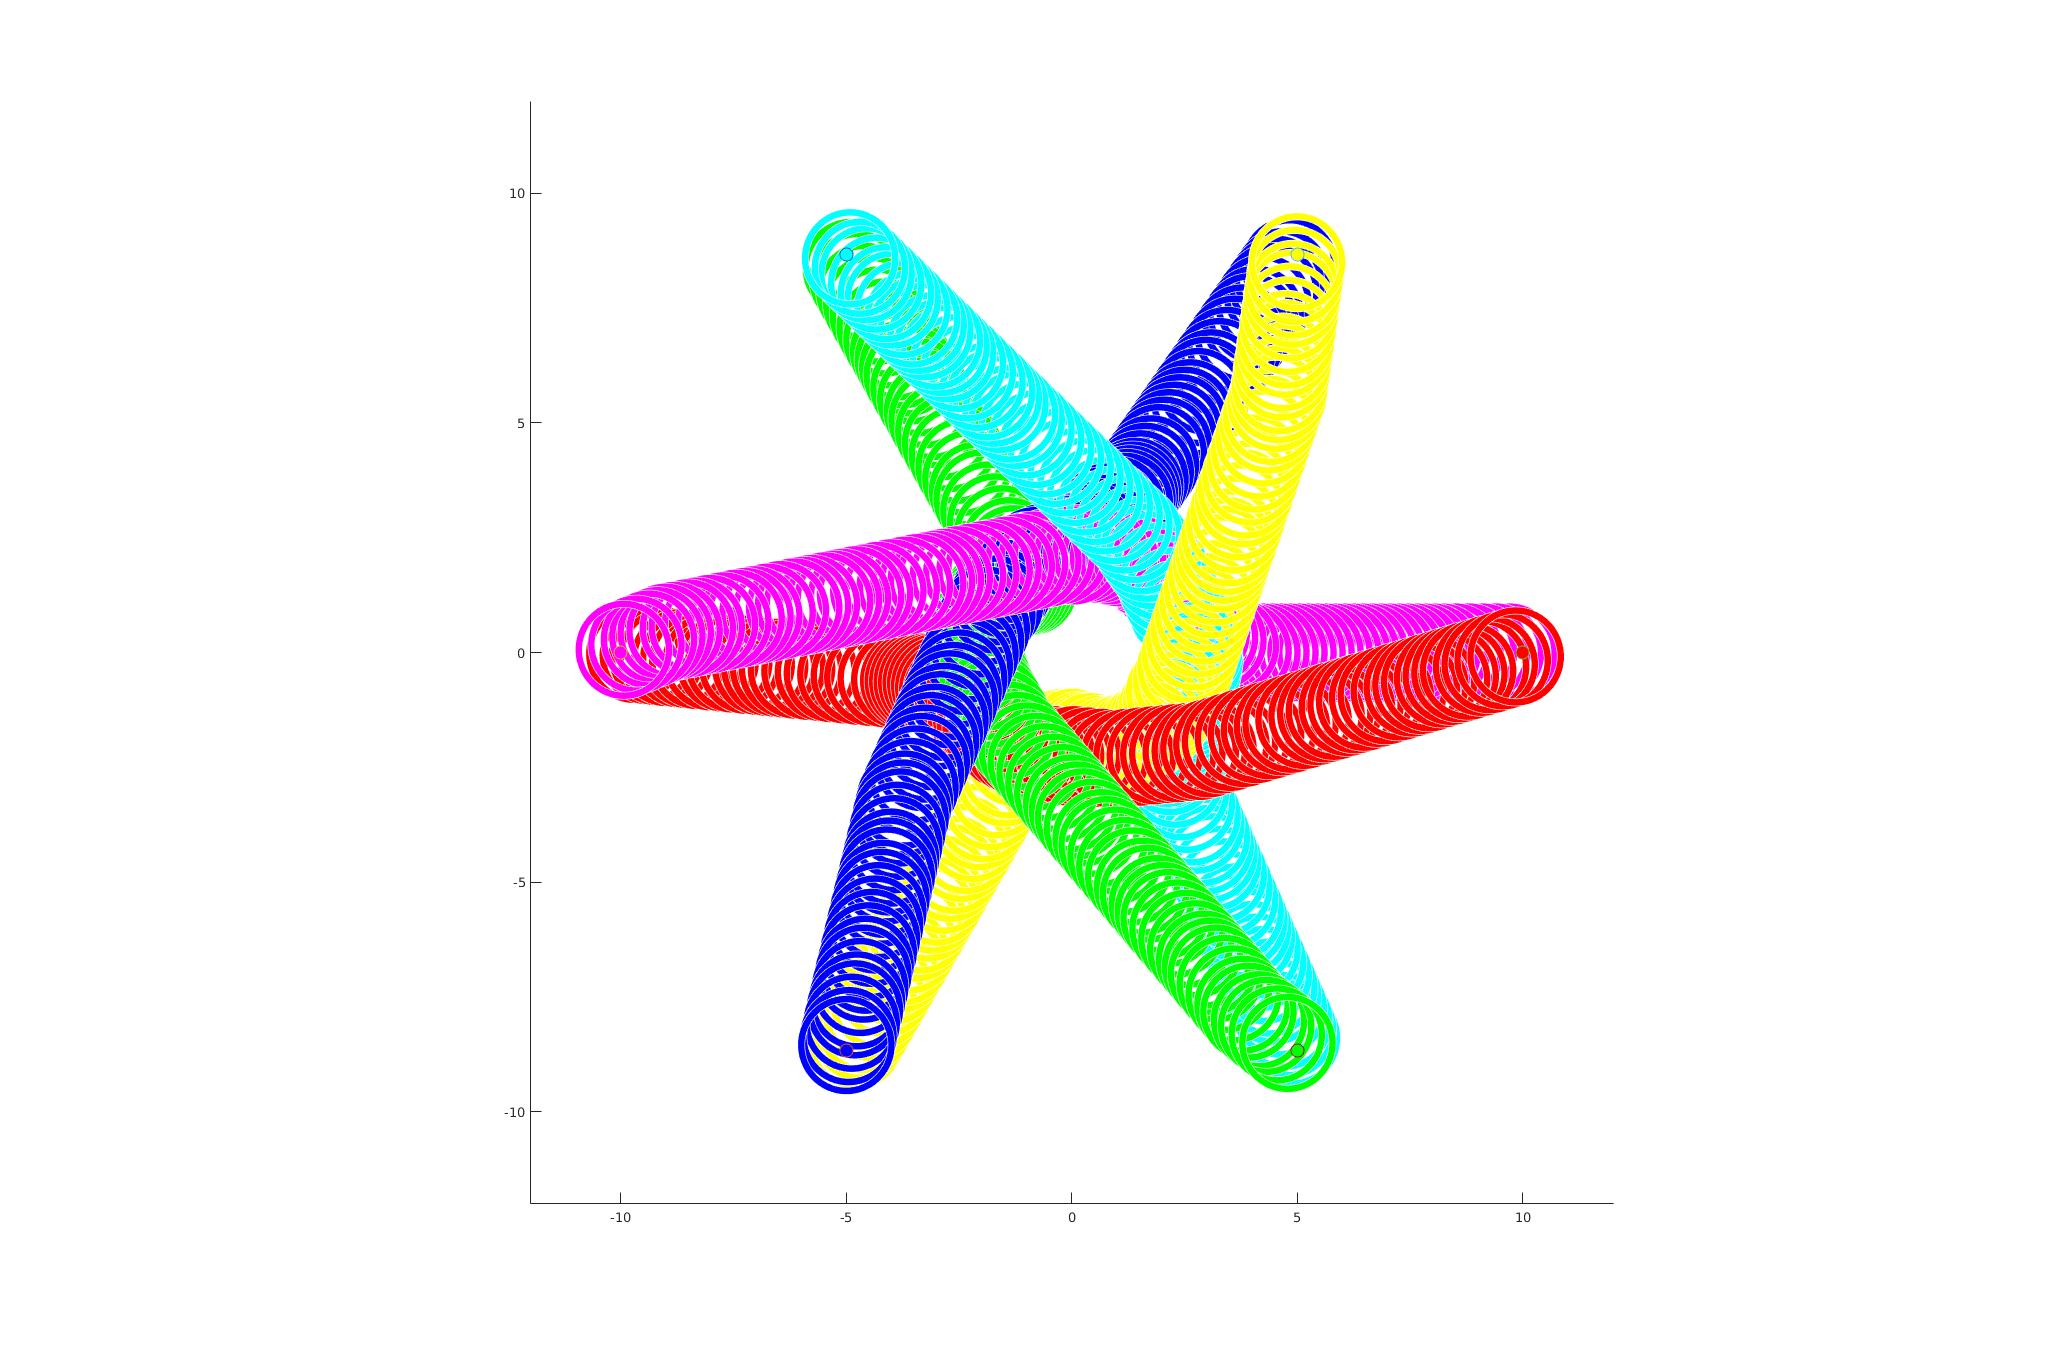
\includegraphics[width=.48\columnwidth]{6tau}} \\

\subfloat[Tre agenti di raggio 1]
{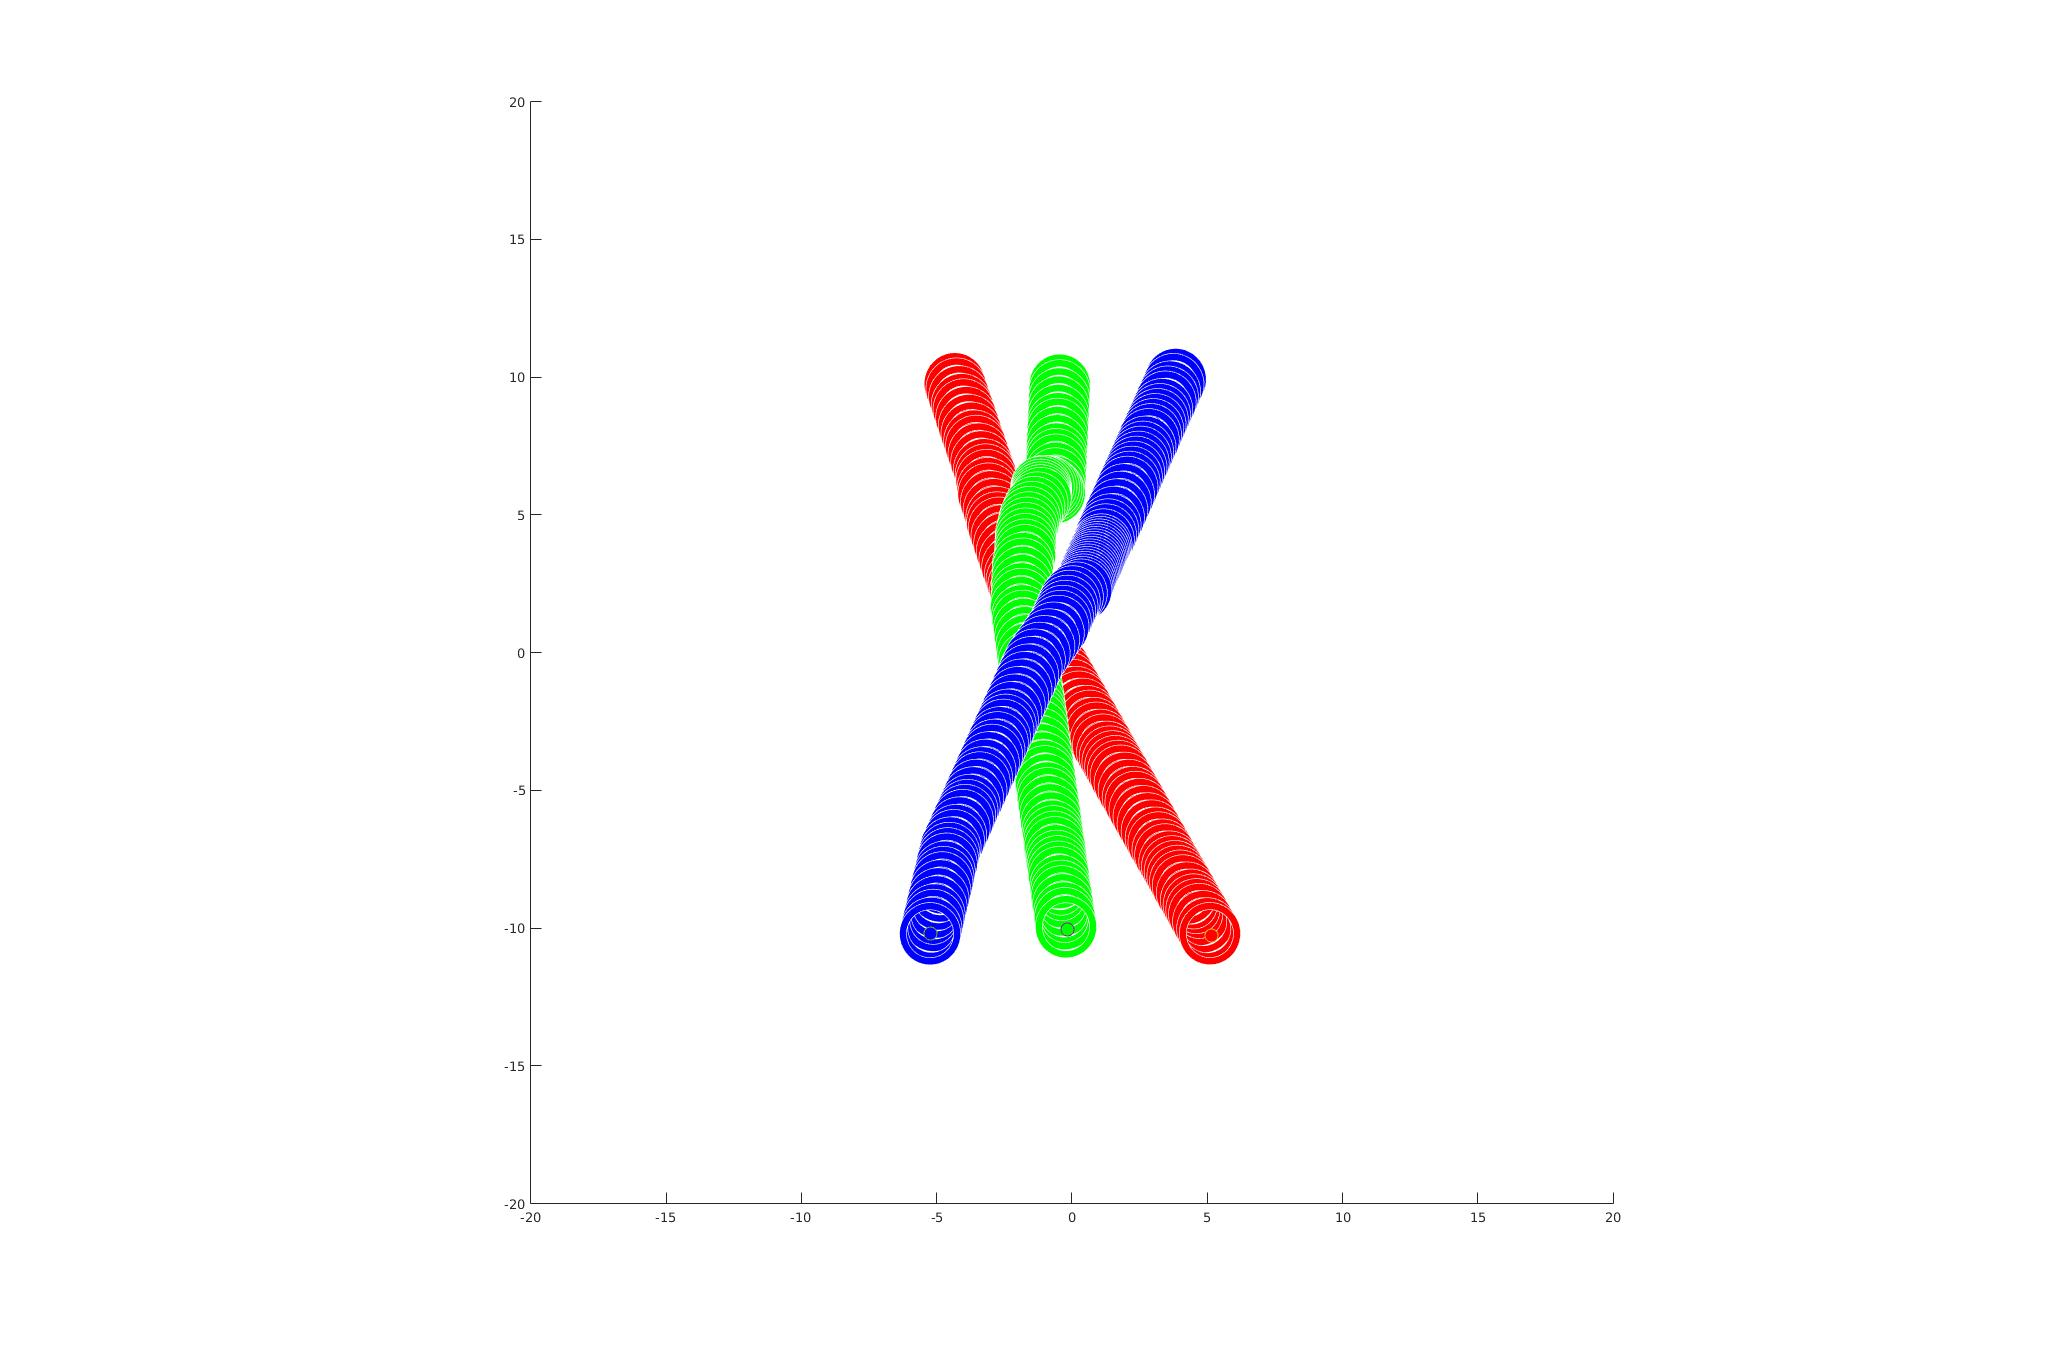
\includegraphics[width=.48\columnwidth]{3Xtau}}
\caption[a,b,c,d dei risulati della simulazione con $\tau$]{Stampa delle traiettorie della simulazione con $\tau$}
\label{fig:}
\end{figure}



% !TEX encoding = UTF-8
% !TEX TS-program = pdflatex
% !TEX root = ../Tesi.tex
% !TEX spellcheck = it-IT

%************************************************
\chapter{Bibliografia}
\label{cap:bib}
%************************************************

\begin{itemize}

\item P. Fiorini, Z. Shiller. Motion planning in dynamic environments using Velocity Obstacles. Int.
Journal of Robotics Research 17(7), pp. 760-772, 1998.

 \item J. van den Berg, M. Lin, D. Manocha. Reciprocal Velocity Obstacles for real-time multi-agent
navigation. IEEE Int. Conf. on Robotics and Automation, pp. 1928–1935, 2008

 \item J. Snape, J. van den Berg, S. Guy, D. Manocha. Independent navigation of multiple mobile
robots with hybrid reciprocal velocity obstacles. IEEE/RSJ Int. Conf. Intell. Robot. Syst.,
2009.

\item Jur van den Berg, Stephen J. Guy, Ming C. Lin, and Dinesh Manocha, “Reciprocal n-body collision avoidance,” in Cédric Pradalier, Roland Siegwart, and Gerhard Hirzinger (eds.), Robotics Research: The 14th International Symposium ISRR, Springer Tracts in Advanced Robotics, vol. 70, Springer-Verlag, Berlin/Heidelberg, Germany, May 7, 2011, pp. 3-19.

\end{itemize}



%\appendix

% *****************************************************************
% Materiale finale
%******************************************************************
%\backmatter
%% !TEX encoding = UTF-8
% !TEX TS-program = pdflatex
% !TEX root = ../Tesi.tex
% !TEX spellcheck = it-IT

%************************************************
\chapter{Bibliografia}
\label{cap:bib}
%************************************************

\begin{itemize}

\item P. Fiorini, Z. Shiller. Motion planning in dynamic environments using Velocity Obstacles. Int.
Journal of Robotics Research 17(7), pp. 760-772, 1998.

 \item J. van den Berg, M. Lin, D. Manocha. Reciprocal Velocity Obstacles for real-time multi-agent
navigation. IEEE Int. Conf. on Robotics and Automation, pp. 1928–1935, 2008

 \item J. Snape, J. van den Berg, S. Guy, D. Manocha. Independent navigation of multiple mobile
robots with hybrid reciprocal velocity obstacles. IEEE/RSJ Int. Conf. Intell. Robot. Syst.,
2009.

\item Jur van den Berg, Stephen J. Guy, Ming C. Lin, and Dinesh Manocha, “Reciprocal n-body collision avoidance,” in Cédric Pradalier, Roland Siegwart, and Gerhard Hirzinger (eds.), Robotics Research: The 14th International Symposium ISRR, Springer Tracts in Advanced Robotics, vol. 70, Springer-Verlag, Berlin/Heidelberg, Germany, May 7, 2011, pp. 3-19.

\end{itemize}
%\input{MaterialeInizialeFinale/Dichiarazione}
\end{document}
